
\documentclass[a4paper,11pt]{article}
\usepackage[a4paper, margin=8em]{geometry}

% usa i pacchetti per la scrittura in italiano
\usepackage[french,italian]{babel}
\usepackage[T1]{fontenc}
\usepackage[utf8]{inputenc}
\frenchspacing 

% usa i pacchetti per la formattazione matematica
\usepackage{amsmath, amssymb, amsthm, amsfonts}

% usa altri pacchetti
\usepackage{gensymb}
\usepackage{hyperref}
\usepackage{standalone}

% cose fluttuanti
\usepackage{float}

% imposta il titolo
\title{Appunti Fondamenti di Automatica}
\author{Luca Seggiani}
\date{2025}

% disegni
\usepackage{pgfplots}
\pgfplotsset{width=10cm,compat=1.9}

% imposta lo stile
% usa helvetica
\usepackage[scaled]{helvet}
% usa palatino
\usepackage{palatino}
% usa un font monospazio guardabile
\usepackage{lmodern}

% tikz in sans
\tikzset{every picture/.style={/utils/exec={\sffamily}}}

\renewcommand{\rmdefault}{ppl}
\renewcommand{\sfdefault}{phv}
\renewcommand{\ttdefault}{lmtt}

% circuiti
\usepackage{circuitikz}
\usetikzlibrary{babel}

% disponi il titolo
\makeatletter
\renewcommand{\maketitle} {
	\begin{center} 
		\begin{minipage}[t]{.8\textwidth}
			\textsf{\huge\bfseries \@title} 
		\end{minipage}%
		\begin{minipage}[t]{.2\textwidth}
			\raggedleft \vspace{-1.65em}
			\textsf{\small \@author} \vfill
			\textsf{\small \@date}
		\end{minipage}
		\par
	\end{center}

	\thispagestyle{empty}
	\pagestyle{fancy}
}
\makeatother

% disponi teoremi
\usepackage{tcolorbox}
\newtcolorbox[auto counter, number within=section]{theorem}[2][]{%
	colback=blue!10, 
	colframe=blue!40!black, 
	sharp corners=northwest,
	fonttitle=\sffamily\bfseries, 
	title=Teorema~\thetcbcounter: #2, 
	#1
}

% disponi definizioni
\newtcolorbox[auto counter, number within=section]{definition}[2][]{%
	colback=red!10,
	colframe=red!40!black,
	sharp corners=northwest,
	fonttitle=\sffamily\bfseries,
	title=Definizione~\thetcbcounter: #2,
	#1
}

% disponi problemi
\newtcolorbox[auto counter, number within=section]{problem}[2][]{%
	colback=green!10,
	colframe=green!40!black,
	sharp corners=northwest,
	fonttitle=\sffamily\bfseries,
	title=Problema~\thetcbcounter: #2,
	#1
}

% disponi codice
\usepackage{listings}
\usepackage[table]{xcolor}

\definecolor{codegreen}{rgb}{0,0.6,0}
\definecolor{codegray}{rgb}{0.5,0.5,0.5}
\definecolor{codepurple}{rgb}{0.58,0,0.82}
\definecolor{backcolour}{rgb}{0.95,0.95,0.92}

\lstdefinestyle{codestyle}{
		backgroundcolor=\color{black!5}, 
		commentstyle=\color{codegreen},
		keywordstyle=\bfseries\color{magenta},
		numberstyle=\sffamily\tiny\color{black!60},
		stringstyle=\color{green!50!black},
		basicstyle=\ttfamily\footnotesize,
		breakatwhitespace=false,         
		breaklines=true,                 
		captionpos=b,                    
		keepspaces=true,                 
		numbers=left,                    
		numbersep=5pt,                  
		showspaces=false,                
		showstringspaces=false,
		showtabs=false,                  
		tabsize=2
}

\lstdefinestyle{shellstyle}{
		backgroundcolor=\color{black!5}, 
		basicstyle=\ttfamily\footnotesize\color{black}, 
		commentstyle=\color{black}, 
		keywordstyle=\color{black},
		numberstyle=\color{black!5},
		stringstyle=\color{black}, 
		showspaces=false,
		showstringspaces=false, 
		showtabs=false, 
		tabsize=2, 
		numbers=none, 
		breaklines=true
}

\lstdefinelanguage{javascript}{
	keywords={typeof, new, true, false, catch, function, return, null, catch, switch, var, if, in, while, do, else, case, break},
	keywordstyle=\color{blue}\bfseries,
	ndkeywords={class, export, boolean, throw, implements, import, this},
	ndkeywordstyle=\color{darkgray}\bfseries,
	identifierstyle=\color{black},
	sensitive=false,
	comment=[l]{//},
	morecomment=[s]{/*}{*/},
	commentstyle=\color{purple}\ttfamily,
	stringstyle=\color{red}\ttfamily,
	morestring=[b]',
	morestring=[b]"
}

% disponi sezioni
\usepackage{titlesec}

\titleformat{\section}
	{\sffamily\Large\bfseries} 
	{\thesection}{1em}{} 
\titleformat{\subsection}
	{\sffamily\large\bfseries}   
	{\thesubsection}{1em}{} 
\titleformat{\subsubsection}
	{\sffamily\normalsize\bfseries} 
	{\thesubsubsection}{1em}{}

% disponi alberi
\usepackage{forest}

\forestset{
	rectstyle/.style={
		for tree={rectangle,draw,font=\large\sffamily}
	},
	roundstyle/.style={
		for tree={circle,draw,font=\large}
	}
}

% disponi algoritmi
\usepackage{algorithm}
\usepackage{algorithmic}
\makeatletter
\renewcommand{\ALG@name}{Algoritmo}
\makeatother

% disponi numeri di pagina
\usepackage{fancyhdr}
\fancyhf{} 
\fancyfoot[L]{\sffamily{\thepage}}

\makeatletter
\fancyhead[L]{\raisebox{1ex}[0pt][0pt]{\sffamily{\@title \ \@date}}} 
\fancyhead[R]{\raisebox{1ex}[0pt][0pt]{\sffamily{\@author}}}
\makeatother

\begin{document}

\pagestyle{fancy}
\thispagestyle{empty}
\renewcommand{\thispagestyle}[1]{}

\maketitle

\documentclass[a4paper,11pt]{article}
\usepackage[a4paper, margin=8em]{geometry}

% usa i pacchetti per la scrittura in italiano
\usepackage[french,italian]{babel}
\usepackage[T1]{fontenc}
\usepackage[utf8]{inputenc}
\frenchspacing 

% usa i pacchetti per la formattazione matematica
\usepackage{amsmath, amssymb, amsthm, amsfonts}

% usa altri pacchetti
\usepackage{gensymb}
\usepackage{hyperref}
\usepackage{standalone}

% imposta il titolo
\title{Appunti Fondamenti di Automatica}
\author{Luca Seggiani}
\date{2025}

% disegni
\usepackage{pgfplots}
\pgfplotsset{width=10cm,compat=1.9}

% imposta lo stile
% usa helvetica
\usepackage[scaled]{helvet}
% usa palatino
\usepackage{palatino}
% usa un font monospazio guardabile
\usepackage{lmodern}

% tikz in sans
\tikzset{every picture/.style={/utils/exec={\sffamily}}}

\renewcommand{\rmdefault}{ppl}
\renewcommand{\sfdefault}{phv}
\renewcommand{\ttdefault}{lmtt}

% disponi il titolo
\makeatletter
\renewcommand{\maketitle} {
	\begin{center} 
		\begin{minipage}[t]{.8\textwidth}
			\textsf{\huge\bfseries \@title} 
		\end{minipage}%
		\begin{minipage}[t]{.2\textwidth}
			\raggedleft \vspace{-1.65em}
			\textsf{\small \@author} \vfill
			\textsf{\small \@date}
		\end{minipage}
		\par
	\end{center}

	\thispagestyle{empty}
	\pagestyle{fancy}
}
\makeatother

% disponi teoremi
\usepackage{tcolorbox}
\newtcolorbox[auto counter, number within=section]{theorem}[2][]{%
	colback=blue!10, 
	colframe=blue!40!black, 
	sharp corners=northwest,
	fonttitle=\sffamily\bfseries, 
	title=Teorema~\thetcbcounter: #2, 
	#1
}

% disponi definizioni
\newtcolorbox[auto counter, number within=section]{definition}[2][]{%
	colback=red!10,
	colframe=red!40!black,
	sharp corners=northwest,
	fonttitle=\sffamily\bfseries,
	title=Definizione~\thetcbcounter: #2,
	#1
}

% disponi problemi
\newtcolorbox[auto counter, number within=section]{problem}[2][]{%
	colback=green!10,
	colframe=green!40!black,
	sharp corners=northwest,
	fonttitle=\sffamily\bfseries,
	title=Problema~\thetcbcounter: #2,
	#1
}

% disponi codice
\usepackage{listings}
\usepackage[table]{xcolor}

\lstdefinestyle{codestyle}{
		backgroundcolor=\color{black!5}, 
		commentstyle=\color{codegreen},
		keywordstyle=\bfseries\color{magenta},
		numberstyle=\sffamily\tiny\color{black!60},
		stringstyle=\color{green!50!black},
		basicstyle=\ttfamily\footnotesize,
		breakatwhitespace=false,         
		breaklines=true,                 
		captionpos=b,                    
		keepspaces=true,                 
		numbers=left,                    
		numbersep=5pt,                  
		showspaces=false,                
		showstringspaces=false,
		showtabs=false,                  
		tabsize=2
}

\lstdefinestyle{shellstyle}{
		backgroundcolor=\color{black!5}, 
		basicstyle=\ttfamily\footnotesize\color{black}, 
		commentstyle=\color{black}, 
		keywordstyle=\color{black},
		numberstyle=\color{black!5},
		stringstyle=\color{black}, 
		showspaces=false,
		showstringspaces=false, 
		showtabs=false, 
		tabsize=2, 
		numbers=none, 
		breaklines=true
}

\lstdefinelanguage{javascript}{
	keywords={typeof, new, true, false, catch, function, return, null, catch, switch, var, if, in, while, do, else, case, break},
	keywordstyle=\color{blue}\bfseries,
	ndkeywords={class, export, boolean, throw, implements, import, this},
	ndkeywordstyle=\color{darkgray}\bfseries,
	identifierstyle=\color{black},
	sensitive=false,
	comment=[l]{//},
	morecomment=[s]{/*}{*/},
	commentstyle=\color{purple}\ttfamily,
	stringstyle=\color{red}\ttfamily,
	morestring=[b]',
	morestring=[b]"
}

% disponi sezioni
\usepackage{titlesec}

\titleformat{\section}
	{\sffamily\Large\bfseries} 
	{\thesection}{1em}{} 
\titleformat{\subsection}
	{\sffamily\large\bfseries}   
	{\thesubsection}{1em}{} 
\titleformat{\subsubsection}
	{\sffamily\normalsize\bfseries} 
	{\thesubsubsection}{1em}{}

% disponi alberi
\usepackage{forest}

\forestset{
	rectstyle/.style={
		for tree={rectangle,draw,font=\large\sffamily}
	},
	roundstyle/.style={
		for tree={circle,draw,font=\large}
	}
}

% disponi algoritmi
\usepackage{algorithm}
\usepackage{algorithmic}
\makeatletter
\renewcommand{\ALG@name}{Algoritmo}
\makeatother

% disponi numeri di pagina
\usepackage{fancyhdr}
\fancyhf{} 
\fancyfoot[L]{\sffamily{\thepage}}

\makeatletter
\fancyhead[L]{\raisebox{1ex}[0pt][0pt]{\sffamily{\@title \ \@date}}} 
\fancyhead[R]{\raisebox{1ex}[0pt][0pt]{\sffamily{\@author}}}
\makeatother

\begin{document}

% sezione (data)
\section{Lezione del 25-02-25}

% stili pagina
\thispagestyle{empty}
\pagestyle{fancy}

% testo
\subsubsection{Introduzione al corso}
Il corso di fondamenti di automatica introduce i concetti di base dell'automazione:
\begin{enumerate}
	\item Introduzione all'automazione;
	\item Modellistica matematica (variabili di stato, trasformata di Laplace, ecc...);
	\item Analisi dei sistemi dinamici (funzioni di trasferimento, ecc...);
	\item Strumenti per l'analisi dei sistemi dinamici (diagrammi di Bode, Nyquist, ecc...);
	\item Sistemi di controllo (PID, ecc...)
\end{enumerate}

\subsection{Introduzione all'automazione}
L'automazione si può intendere come la capacità di eseguire un compito \textit{in modo automatico}.
Per ogni \textit{compito} visto durante il corso si creerà un modello matematico, e un sistema capace di eseguirlo in maniera autonoma, senza l'intervento di esterni.

Elemento chiave nei sistemi che verranno studiati sarà il \textbf{feedback}, in italiano \textit{retroazione}, che rappresenta l'informazione che possiamo prendere indietro dal sistema in modo da influenzare i sistemi di controllo automatico.

\subsubsection{Fasi di sviluppo}
Il termine inglese \textit{"automation"} viene introdotto come contrazione di \textit{"automatic production"} dalla Ford Motor Company nel 1947 per denominare l'insieme di apparati di movimentazione automatica installati nelle loro linee di produzione.

Possiamo tracciare diverse fasi di sviluppo della disciplina dell'automazione:
\begin{enumerate}
	\item \textbf{Prima rivoluzione industriale} ($\sim$1780): \\
		Vengono introdotti i primi strumenti meccanici di produzione (macchine a vapore, ecc...).
	\item \textbf{Seconda rivoluzione industriale} ($\sim$1870): \\
		Si organizza il lavoro in catene di produzione sfruttando l'energia elettrica (catena Ford, ecc...).
	\item \textbf{Terza rivoluzione industriale} ($\sim$1970): \\ 
		Si automatizza il processo di produzione grazie a sistemi IT ed elettronici (PLC, ecc...).
	\item \textbf{Quarta rivoluzione industriale} ($\sim$2010): \\
		Prodotti e processi interconnessi grazie all'IoT e a tecnologie digitali (industria 4.0, ecc...).
\end{enumerate}

\subsubsection{Tecnologie abilitanti}
Possiamo individuare alcune macroaree dell'automazione moderna, in ambito (perlopiù) industriale:
\begin{itemize}
	\item Tecniche di produzione avanzate (stampa 3D (additiva), ecc...);
	\item Realtà aumentata;
	\item Simulazione;
	\item Sviluppo orizzontale e verticale;
	\item IoT industriale (IIoT);
	\item Cloud computing;
	\item Cybersecurity;
	\item Big data analytics.
\end{itemize}

\subsection{Modellistica matematica}
\subsubsection{Sistemi}
Veniamo quindi alle tecniche che ci permettono di studiare matematicamente un dato \textbf{sistema}.
\begin{definition}{Sistema}
	Un sistema è un insieme di parti interconnesse e interagenti che formano un insieme più grande e complesso.
\end{definition}

Di un sistema ci interessano gli \textbf{ingressi}, cioè cosa \textit{entra} nel sistema, e le \textbf{uscite}, cioè cosa \textit{esce} dal sistema.
Ogni sistema è caratterizzato poi da un certo livello di \textbf{disturbo}.
L'idea è spesso quella di \textit{inseguire} gli ingressi e \textit{reiettare} i disturbi.

\subsubsection{Sistemi dinamici}
Ad interessarci in particolare sono  sistemi \textbf{dinamici}.
\begin{definition}{Sistema dinamico}
	Un sistema si dice dinamico quando le sue grandezze si evolvono nel tempo.
\end{definition}

Le grandezze di un sistema dinamico (le uscite e lo stato interno) sono quindi caratterizzate da funzioni con variabile tempo, che quindi \textit{variano} nel tempo e interagiscono con l'ambiente esterno.

Solitamente i sistemi dinamici sono costituiti da più sottosistemi che interagiscono fra di loro.

\par\medskip

Incontriamo diversi problemi nello studio dei sistemi:
\begin{itemize}
	\item Se è ignoto il sistema, abbiamo il problema della \textbf{modellistica}, che consiste nel creare un modello matematico del sistema, e quindi del suo comportamento;
	\item Se è ignota l'uscita, abbiamo il problema della \textbf{simulazione}, che consiste nel simulare la risposta del sistema, nel tempo, in base alla variazione degli ingressi;
	\item Se conosciamo il sistema e la sua uscita, abbiamo il problema del \textbf{controllo}, che consiste nello studiare come agire \textit{dall'esterno} su un sistema per modificarne la naturale evoluzione ed ottenere un comportamento desiderato.
		Ad agire sul sistema sarà spesso un altro sistema, detto \textbf{sistema di controllo}, che produrrà gli ingressi del sistema vero e proprio sulla base di dati \textbf{comandi}.
\end{itemize}

\subsubsection{Diagrammi a blocchi}
Rappresentiamo i modelli che facciamo sistemi attraverso diagrammi a \textit{"scatole"} o a \textbf{blocchi}:

\begin{center}
	\begin{tikzpicture}
		\draw[fill=cyan] (0,0) rectangle (2, 1);
		\draw[-stealth] (-2, 0.5) -> (0, 0.5);
		\draw[-stealth] (2, 0.5) -> (4, 0.5);
		\draw[-stealth] (1, 2) -> (1, 1);

		\node at (1, 0.5) {Sistema};
		\node at (-1, 0.8) {Ingressi};
		\node at (3, 0.8) {Uscite};
		\node at (1, 2.3) {Disturbi};
	\end{tikzpicture}
\end{center} 

La scatola sistema è spesso caratterizzata da una certa funzione matematica $f(u, \xi, \theta)$, dove $\xi$ rappresenta i disturbi e $\theta$ i parametri del modello.
Gli ingressi e le uscite saranno quindi rappresentati da variabili $u$ e $y$, con $y = f(u, \xi, \theta)$. 
Notiamo che la funzione che rappresenta il sistema ha la variabile di ingresso $u$ come argomento.

\begin{center}
	\begin{tikzpicture}
		\draw (0,0) rectangle (2, 1);
		\draw[-stealth] (-2, 0.5) -> (0, 0.5);
		\draw[-stealth] (2, 0.5) -> (4, 0.5);
		\node at (1, 0.5) {$f(u, \xi, \theta)$};
		\node at (-1, 0.7) {$u$};
		\node at (3, 0.7) {$y$};
	\end{tikzpicture}
\end{center}

\subsubsection{Proprietà dei sistemi dinamici}
Notiamo alcune proprietà dei sistemi dinamici:
\begin{itemize}
	\item Questi devono essere \textbf{causali}, cioè l'uscita non deve dipendere da valori futuri dell'ingresso: se l'uscita è rappresentata da $v(t)$ e l'ingresso da $u(t)$, si ha che $v(t)$ dipende da $u(t)$ solo per $t < t_0$ con $t_0$ l'istante corrente;
	\item Possono essere sia \textbf{stocastici} che \textbf{deterministici}, se sono presenti o meno fenomeni aleatori nel legame ingresso uscita. Il corso in particolare tratterà di sistemi \textit{deterministici};
\end{itemize}

\subsection{Modellistica di sistemi}
Vediamo gli approcci più comuni alla modellazione di sistemi dinamici.

\subsubsection{Modello a scatola nera}
Possiamo adottare un approccio sperimentale (o \textit{induttivo}) alla modellistica di un sistema, considerandolo come una \textbf{scatola nera} (\textit{black box}) 

\begin{center}
	\begin{tikzpicture}
		% scatola nera
		\draw[fill=darkgray] (0,0) rectangle (2, 1);
		\node[text width=1.5cm, text centered, color=white] at (1, 0.5) {Scatola nera};
		% misura
		\draw (4,0) rectangle (6, 1);
		\node at (5, 0.5) {Misura};
		
		\draw[-stealth] (-2, 0.5) -> (0, 0.5);
		\draw[-stealth] (2, 0.5) -> (4, 0.5);
		
		\draw[-stealth] (3, -2) -> (3, -3);

		\draw (-1, 0.5) -> (-1, -1.5);
		\draw (5, 0) -> (5, -1.5);
		\draw[-stealth] (-1, -1.5) -> (2, -1.5);
		\draw[-stealth] (5, -1.5) -> (4, -1.5);

		% tabelle
		\draw (2,-2) rectangle (4, -1);
		\node at (3, -1.5) {Tabelle};
		% fitting
		\draw (2,-4) rectangle (4, -3);
		\node at (3, -3.5) {Fitting};
		
		% modello
		\draw[fill=lime] (5,-4) rectangle (7, -3);
		\node at (6, -3.5) {Modello};

		\draw[-stealth] (4, -3.5) -> (5, -3.5); 

		\node at (-1, 0.8) {Ingressi};
	\end{tikzpicture}
\end{center}

L'idea è quella di studiare il comportamento del sistema in risposta a diversi stimoli, e costruire un'associazione fra stimolo e risposta corrispondente.
Il problema (\textit{fitting}) da qui in poi sarà quello di trovare una certa funzione che approssima, per quanto possibile, il comportamento del sistema in risposta ai diversi stimoli.
Approcci per il fitting della funzione di risposta possono essere:
\begin{itemize}
	\item Regole stato-azione;
	\item Alberi decisionali;
	\item Regressione lineare;
	\item Modelli statistici;
	\item Reti neurali.
\end{itemize}

Un approccio di questo tipo non richiede alcuna conoscenza del principio di funzionamento interno del sistema (dettagli fisici, tecnici, ecc...), ed è quindi puramente sperimentale.

Notiamo che approcci di questo tipo sono effettivamente alla base delle tecniche di apprendimento automatico.
In questo le reti neurali per l'apprendimento \textit{supervisionato} non sono che una tecnica molto potente per il fitting di varie relazioni ingresso-uscita.

\subsubsection{Modello a scatola bianca}
Un altro approccio è quello analitico (o \textit{deduttivo}).
In questo caso si costruisce un modello astratto del sistema di interesse, e si \textit{valida} confrontandolo col sistema reale, agendo con delle modifiche nel caso di incongruenze. 

\begin{center}
	\begin{tikzpicture}
		% sistema reale
		\draw[fill=cyan] (0,0) rectangle (2, 1);
		\node[text width=1.5cm, text centered] at (1, 0.5) {Sistema reale};
		% modello astratto
		\draw (0,-2) rectangle (2, -1);
		\node[text width=1.5cm, text centered] at (1, -1.5) {Modello astratto};
		
		\draw[-stealth] (-2, 0.5) -> (0, 0.5);
		\draw[-stealth] (2, 0.5) -> (4, 0.5);
		
		\draw (-1, 0.5) -> (-1, -1.5);
		\draw[stealth-] (5, 0) -> (5, -1.5);
		\draw[-stealth] (-1, -1.5) -> (0, -1.5);
		\draw (5, -1.5) -> (2, -1.5);
		
		\draw (5.5, 0) -> (5.5, -1.7);
		\draw[-stealth] (5.5, -1.7) -> (2, -1.7);

		% validazione
		\draw (4,0) rectangle (6, 1);
		\node at (5, 0.5) {Validazione};
		
		\draw[-stealth] (6, 0.5) -> (7, 0.5);

		% modello 
		\draw[fill=lime] (7,0) rectangle (9, 1);
		\node at (8, 0.5) {Modello};

		\node at (-1, 0.8) {Ingressi};
	
		\node at (3.5, -1.9) {Modifica};
	\end{tikzpicture}
\end{center}

Approcci di questo tipo richiedono di ricavare modelli astratti di sistemi, conoscendone quindi le leggi di funzionamento interno.
Per questo sono molto accurati per sistemi ben conosciuti, ma difficili da realizzare altrimenti.

\subsubsection{Modello a scatola grigia}
Un approccio intermedio fra scatola nera e scatola bianca è quello a \textbf{scatola grigia}.
In questo caso assumiamo di conoscere il comportamento generale del sistema, ma di dover identificare parametri specifici.
Si crea quindi un modello a scatola bianca, lasciando vuoti i parametri che non si conoscono (\textit{scatola bianca}). 
Svolgendo varie misurazioni e confrontando i risultati del modello astratto e del sistema reale si andranno poi a determinare nel dettaglio tali parametri (\textit{scatola nera}).

\subsubsection{Approccio pragmatico}
Un approccio pragmatico consiste nello sviluppare un modello a priori, senza considerare necessariamente un sistema reale, e poi adattarlo fino alla convergenza con un sistema veramente esistente.

Dal punto di vista ingegneristico, quento significa ipotizzare un modello per un sistema ideale, che andiamo quindi a definire in maniera astratta, e poi ad implementare nella realtà cercando di avvicinarci il più possibile all'idea originale. 

\end{document}


\documentclass[a4paper,11pt]{article}
\usepackage[a4paper, margin=8em]{geometry}

% usa i pacchetti per la scrittura in italiano
\usepackage[french,italian]{babel}
\usepackage[T1]{fontenc}
\usepackage[utf8]{inputenc}
\frenchspacing 

% usa i pacchetti per la formattazione matematica
\usepackage{amsmath, amssymb, amsthm, amsfonts}

% usa altri pacchetti
\usepackage{gensymb}
\usepackage{hyperref}
\usepackage{standalone}

% imposta il titolo
\title{Appunti Fondamenti di Automatica}
\author{Luca Seggiani}
\date{2025}

% disegni
\usepackage{pgfplots}
\pgfplotsset{width=10cm,compat=1.9}

% imposta lo stile
% usa helvetica
\usepackage[scaled]{helvet}
% usa palatino
\usepackage{palatino}
% usa un font monospazio guardabile
\usepackage{lmodern}

% tikz in sans
\tikzset{every picture/.style={/utils/exec={\sffamily}}}

\renewcommand{\rmdefault}{ppl}
\renewcommand{\sfdefault}{phv}
\renewcommand{\ttdefault}{lmtt}

% circuiti
\usepackage{circuitikz}
\usetikzlibrary{babel}

% disponi il titolo
\makeatletter
\renewcommand{\maketitle} {
	\begin{center} 
		\begin{minipage}[t]{.8\textwidth}
			\textsf{\huge\bfseries \@title} 
		\end{minipage}%
		\begin{minipage}[t]{.2\textwidth}
			\raggedleft \vspace{-1.65em}
			\textsf{\small \@author} \vfill
			\textsf{\small \@date}
		\end{minipage}
		\par
	\end{center}

	\thispagestyle{empty}
	\pagestyle{fancy}
}
\makeatother

% disponi teoremi
\usepackage{tcolorbox}
\newtcolorbox[auto counter, number within=section]{theorem}[2][]{%
	colback=blue!10, 
	colframe=blue!40!black, 
	sharp corners=northwest,
	fonttitle=\sffamily\bfseries, 
	title=Teorema~\thetcbcounter: #2, 
	#1
}

% disponi definizioni
\newtcolorbox[auto counter, number within=section]{definition}[2][]{%
	colback=red!10,
	colframe=red!40!black,
	sharp corners=northwest,
	fonttitle=\sffamily\bfseries,
	title=Definizione~\thetcbcounter: #2,
	#1
}

% disponi problemi
\newtcolorbox[auto counter, number within=section]{problem}[2][]{%
	colback=green!10,
	colframe=green!40!black,
	sharp corners=northwest,
	fonttitle=\sffamily\bfseries,
	title=Problema~\thetcbcounter: #2,
	#1
}

% disponi codice
\usepackage{listings}
\usepackage[table]{xcolor}

\lstdefinestyle{codestyle}{
		backgroundcolor=\color{black!5}, 
		commentstyle=\color{codegreen},
		keywordstyle=\bfseries\color{magenta},
		numberstyle=\sffamily\tiny\color{black!60},
		stringstyle=\color{green!50!black},
		basicstyle=\ttfamily\footnotesize,
		breakatwhitespace=false,         
		breaklines=true,                 
		captionpos=b,                    
		keepspaces=true,                 
		numbers=left,                    
		numbersep=5pt,                  
		showspaces=false,                
		showstringspaces=false,
		showtabs=false,                  
		tabsize=2
}

\lstdefinestyle{shellstyle}{
		backgroundcolor=\color{black!5}, 
		basicstyle=\ttfamily\footnotesize\color{black}, 
		commentstyle=\color{black}, 
		keywordstyle=\color{black},
		numberstyle=\color{black!5},
		stringstyle=\color{black}, 
		showspaces=false,
		showstringspaces=false, 
		showtabs=false, 
		tabsize=2, 
		numbers=none, 
		breaklines=true
}

\lstdefinelanguage{javascript}{
	keywords={typeof, new, true, false, catch, function, return, null, catch, switch, var, if, in, while, do, else, case, break},
	keywordstyle=\color{blue}\bfseries,
	ndkeywords={class, export, boolean, throw, implements, import, this},
	ndkeywordstyle=\color{darkgray}\bfseries,
	identifierstyle=\color{black},
	sensitive=false,
	comment=[l]{//},
	morecomment=[s]{/*}{*/},
	commentstyle=\color{purple}\ttfamily,
	stringstyle=\color{red}\ttfamily,
	morestring=[b]',
	morestring=[b]"
}

% disponi sezioni
\usepackage{titlesec}

\titleformat{\section}
	{\sffamily\Large\bfseries} 
	{\thesection}{1em}{} 
\titleformat{\subsection}
	{\sffamily\large\bfseries}   
	{\thesubsection}{1em}{} 
\titleformat{\subsubsection}
	{\sffamily\normalsize\bfseries} 
	{\thesubsubsection}{1em}{}

% disponi alberi
\usepackage{forest}

\forestset{
	rectstyle/.style={
		for tree={rectangle,draw,font=\large\sffamily}
	},
	roundstyle/.style={
		for tree={circle,draw,font=\large}
	}
}

% disponi algoritmi
\usepackage{algorithm}
\usepackage{algorithmic}
\makeatletter
\renewcommand{\ALG@name}{Algoritmo}
\makeatother

% disponi numeri di pagina
\usepackage{fancyhdr}
\fancyhf{} 
\fancyfoot[L]{\sffamily{\thepage}}

\makeatletter
\fancyhead[L]{\raisebox{1ex}[0pt][0pt]{\sffamily{\@title \ \@date}}} 
\fancyhead[R]{\raisebox{1ex}[0pt][0pt]{\sffamily{\@author}}}
\makeatother

\begin{document}

% sezione (data)
\section{Lezione del 26-02-25}

% stili pagina
\thispagestyle{empty}
\pagestyle{fancy}

% testo
\subsubsection{Modello a stati}
Un possibile approccio alla modellistica di un sistema è la creazione di una \textbf{macchina a stati finiti} (FSM, \textit{Finite State Machine}).

Questo chiaramente porterà alla definizione di un determinato numero di \textbf{stati} in cui il sistema si potrà trovare in qualsiasi momento.
Azioni sul sistema corrisponderanno quindi a \textbf{transizioni} fra uno stato un altro, e ogni transizione comporterà un aggiornamento dell'uscita del sistema.
La risposta del sistema a ogni azione dall'esterno dipende quindi non solo dall'azione, ma dallo stato interno corrente del sistema, che è quindi dotato di \textbf{memoria}.

La modellizzazione con macchine a stati finiti risulta particolarmente utile in informatica, in quanto modellizza molto bene una vasta gamma di sistemi digitali.

\subsection{Modellizzazione a scatola bianca semplice}
Iniziamo a vedere come si possono modellizzare sistemi fisici attraverso approcci a scatola bianca. 

\subsubsection{Esempio: serbatoio a galleggiante}
Prendiamo il caso di un serbatoio, con in in ingresso un rubinetto di portata $p$, di cui si vuole tenere costante il livello del liquido ad un valore $\overline{h}$. 
Sistemi di questo tipo sono comuni in diversi contesti, fra cui gli sciaquoni dei water e le vaschette dei carburatori per motori a scoppio.

Chiamiamo il livello del liquido ad ogni istante temporale $h(t)$.
Il valore desiderato di tale funzione, che indichiamo come $h_o(t) = \overline{h}$, verrà detto \textbf{segnale di riferimento}.

L'ingresso del sistema su cui vogliamo agire sarà $u(t) = p(t)$, cioè la portata del rubinetto (che modificheremo ad esempio controllando una valvola).

Nel caso non ci siano disturbi, ergo tutto il liquido immesso nel serbatoio resti nel serbatoio, avremo una variazione di volume $\Delta V$ pari a:
$$
\Delta V = A \cdot (h_1 - h_0) = \int_{t_0}^{t_1} u(\tau) \, d\tau
$$
dove $A$ rappresenta l'area di base del serbatoio.

Da questo si ricava:
$$
A \cdot \frac{dh}{dt} = u(t)
$$

Chiamando $x \leftarrow h$ si otterrà l'equazione differenziale:
$$
x' = \frac{1}{A}u(t)
$$
Di cui chiaramente ci interessa la \textbf{condizione iniziale} $x_0$, cioè il livello del liquido all'istante temporale $t=0$.

\subsubsection{Esempio: circuito di carica di un condensatore}
Prendiamo il circuito formato da un condensatore $C$ posto in serie ad un generatore di corrente $i$:

\begin{center}
	\begin{circuitikz}
		\draw (0, 0) -- (3, 0)
			to[capacitor, v<=$V$] (3, -3)
			-- (0, -3)
			to[current source, i=$i$] (0, 0);
			
	\end{circuitikz}
\end{center}

Avremo che la variazione di carica sulle armature $\Delta q$ varrà:
$$
\Delta q = C \cdot (V_1 - V_0) = \int_{t_0}^{t_1} i(\tau) d \tau \implies C \frac{dV}{dt} = i(t)
$$
da cui si ricava l'equazione differenziale del tutto analoga a prima:
$$
x' = \frac{1}{C} i(t)
$$

L'unica cosa che cambia, rispetto al sistema precedente, sono i nomi delle variabili e le grandezze fisiche che rappresentano.
Dal punto di vista matematico, quindi, possiamo assumere i due sistemi come equivalenti.

\subsubsection{Esempio: legge di Newton}
Vediamo come equazioni analoghe alle precedenti si ricavano in verità da qualsiasi sistema meccanico che obbedisce alla legge di Newton:
$$
F = m a \implies m \frac{dv}{dt} = F(t)
$$
da cui:
$$
x' = \frac{1}{m}F(t)
$$
notando che chiamiamo $x \leftarrow v$ (ci riferiamo alle velocità, non alle posizioni).

\par\smallskip

Gli elementi visti finora non sono altro che \textbf{integratori}, cioè sistemi dinamici che prendono $x'$ e restituiscono $x$ per una certa variabile.

Indichiamo questi come segue:

\begin{center}
	\begin{tikzpicture}
		\draw (0,0) rectangle (1, 1);
		\draw[-stealth] (-2, 0.5) -> (0, 0.5);
		\draw[-stealth] (1, 0.5) -> (3, 0.5);
		\node at (0.5, 0.5) {$\int$};
		\node at (-1, 0.75) {$x'$};
		\node at (2, 0.7) {$x$};
	\end{tikzpicture}
\end{center}

e, se vogliamo, vedremo che nel dominio di Laplace vale la divisione per la variabile $s = \sigma + i \omega$:

\begin{center}
	\begin{tikzpicture}
		\draw (0,0) rectangle (1, 1);
		\draw[-stealth] (-2, 0.5) -> (0, 0.5);
		\draw[-stealth] (1, 0.5) -> (3, 0.5);
		\node at (0.5, 0.5) {$\frac{1}{s}$};
		\node at (-1, 0.75) {$x'$};
		\node at (2, 0.7) {$x$};
	\end{tikzpicture}
\end{center}

\subsection{Sistemi Lineari e Tempo Invarianti (LTI)}
Vediamo un particolare tipo di sistema dinamico:
\begin{definition}{Sistema LTI}
	Un sistema LTI (Lineare e Tempo Invariante) rispetta le seguenti proprietà:
	\begin{itemize}
		\item \textbf{Omogeneità:} se si scala l'ingresso $u(t)$, l'uscita $y(t)$ viene scalata dello stesso fattore:
			$$
				au(t) \implies ay(t)
			$$

		\item \textbf{Sovrapposizione degli effetti:} se un modello ha risposte $y_1(t)$ e $y_2(t)$ a due ingressi qualsiasi $u_1(t)$ e $u_2(t)$, allora la risposta a un ingresso dato dalla combinazione lineare di $u_1(t)$ e $u_2(t)$:
			$$
				u(t) = \alpha_1 u_1(t) + \alpha_2 u_2(t)
			$$

			sarà data ancora da una combinazione lineare delle uscite in risposta ai singoli ingressi:
			$$
				y(t) = \alpha_1 y_1(t) + \alpha_2 y_2(t)
			$$
			
			Notiamo che in questo la sovrapposizione degli effetti non rappresenta altro che la proprietà di \textit{linearità} dei sistemi lineari.
	
		\item \textbf{Tempo invarianza:} iil sistema si comporta allo stesso modo indipendentemente da quando avviene l'azione, cioè nelle equazioni che lo descrivono non vi è una dipendenza esplicita dal tempo.
			Questo significa che un ingresso $u(t - \tau)$ produce un uscita $y(t - \tau)$, cioè solo traslata in tempo:

		\begin{center}
			\begin{tikzpicture}
				\draw (0,0) rectangle (2, 1);
				\draw[-stealth] (-2, 0.5) -> (0, 0.5);
				\draw[-stealth] (2, 0.5) -> (4, 0.5);
				\node at (1, 0.5) {$\mathrm{LTI}$};
				\node at (-1, 0.7) {$u(t - \tau)$};
				\node at (3, 0.7) {$y(t - \tau)$};
			\end{tikzpicture}
		\end{center}
	\end{itemize}
\end{definition}

I sistemi lineari e tempo invarianti ci sono particolarmente utili in quanto sono completamente compresi e facili da risolvere, e riescono a modellizzare in maniera abbastanza accurata una vasta gamma di fenomeni.

\subsection{Modellizzazione a equazioni differenziali lineari}
Estendiamo l'approccio a scatola bianca introducendo formalmente una forma ad \textbf{equazioni differenziali lineari}.

\begin{definition}{Modello a variabili di stato}
	Introduciamo il modello per sistemi a equazioni differenziali lineari:
	\[
		\begin{cases}
			x' = Ax + Bu \\ 
			y = Cx + Du
		\end{cases}
	\]
	dove $u \in \mathbb{R}^r$ è l'\textbf{ingresso} e $x \in \mathbb{R}^n$ è lo \textbf{stato} del sistema.
	$x'$ sarà quindi la variazione dello stato, e $y \in \mathbb{R}^m$ l'uscita del sistema.
\end{definition}

Abbiamo quindi un sistema di equazioni vettoriali differenziali che mettono in relazione fra di loro lo \textit{stato interno presente} $x$, la variazione di stato $x'$, l'ingresso $u$ e l'uscita $y$ del sistema.

Le dimensioni delle matrici che correlano variazione di stato e uscita a stato interno presente e ingresso, cioè le matrici $A, B, C, D$, si ricaveranno dalle dimensioni delle variabili ($r, n$ e $m$):

$$
A \in \mathbb{R}^{n \times n}, \, 
B \in \mathbb{R}^{n \times r}, \, 
C \in \mathbb{R}^{m \times n}, \, 
D \in \mathbb{R}^{m \times r}, \, 
$$

La tempo invarianza del sistema è data proprio dalla tempo invarianza delle matrici, che non hanno il tempo come argomento ma sono costanti.

\subsubsection{Proprietà strutturali}
L'analisi delle matrici $A, B, C, D$ definisce le cosiddette \textbf{proprietà strutturali} del sistema.
Ad esempio abbiamo che:
\begin{itemize}
	\item La matrice $A$ ci dà informazioni riguardo alla proprietà di \textbf{stabilità} del sistema;
	\item Le matrici $A, B$ ci danno informazioni riguardo alla \textbf{controllabilità} del sistema;
	\item Le matrici $A, C$ ci danno informazioni riguardo all'\textbf{osservabilità} del sistema.
\end{itemize}

\subsubsection{Diagramma a blocchi}
Possiamo usare l'operatore integrale definito prima per creare il diagramma a blocchi del sistema a equazioni differenziali linari:

\begin{center}
	\begin{tikzpicture}
		% integratore
		\draw (0,0) rectangle (1, 1);

		% A 
		\draw (0,-1) rectangle (1, -2);
		
		% D
		\draw (0,-3) rectangle (1, -4);
		
		% B 
		\draw (-5,0) rectangle (-4, 1);
		
		% C 
		\draw (3,0) rectangle (4, 1);

		\draw[-stealth] (-2, 0.5) -> (0, 0.5);
		\draw[-stealth] (1, 0.5) -> (3, 0.5);
		
		\draw[-stealth] (-7, 0.5) -> (-5, 0.5);
		\draw[-stealth] (-4, 0.5) -> (-2.1, 0.5);
		
		\draw[-stealth] (4, 0.5) -> (5.9, 0.5);
		\draw[-stealth] (6, 0.5) -> (8, 0.5);

		\draw (2, 0.5) -> (2, -1.5);
		\draw[-stealth] (2, -1.5) -> (1, -1.5);

		\draw (0, -1.5) -> (-2, -1.5);
		\draw[-stealth] (-2, -1.5) -> (-2, 0.4);


		\draw (-6, 0.5) -> (-6, -3.5);
		\draw (-6, -3.5) -> (0, -3.5);

		\draw (1, -3.5) -> (6, -3.5);
		\draw[-stealth] (6, -3.5) -> (6, 0.4);


		\node at (0.5, 0.5) {$\int$};
		\node at (0.5, -1.5) {$A$};
		\node at (0.5, -3.5) {$D$};
		
		\node at (-4.5, 0.5) {$B$};
		\node at (3.5, 0.5) {$C$};

		\node at (-6, 0.75) {$u$};
		\node at (7, 0.75) {$y$};
		
		\node at (-1, 0.75) {$x'$};
		\node at (2, 0.7) {$x$};
	
		% sommatore B - integratore
		\draw[fill=white] (-2, 0.5) circle (0.1);
		
		% sommatore C - uscita 
		\draw[fill=white] (6, 0.5) circle (0.1);

	\end{tikzpicture}
\end{center}

Notando che il simbolo $\circ$ rappresenta una somma.

\subsubsection{Esempio: partitore di tensione}
Vediamo per il modello introdotto l'esempio del \textit{partitore resistivo} o partitore di tensione.

\begin{center}
	\begin{circuitikz}
		\draw (0,0) -- (2,0)
			to[resistor, R=$R_1$] (2,-2)
			to[resistor, R=$R_2$] (2,-4) node[ground]{};

		\draw (2, -2) -- (4, -2);

		\node at (-0.5, 0) {$V_{in}$};
		\node at (4.5, -2) {$V_{out}$};
	\end{circuitikz}
\end{center}

La relazione che otteniamo, dalla legge del partitore di tensione, per il voltaggio, è:
$$
V_{out} = \frac{R_2}{R_1 + R_2} V_{in} = \alpha V_{in}, \quad \alpha = \frac{R_1}{R_1 + R_2}
$$

da cui:
$$
A = B = C = 0, \ D = \alpha 
$$ # rivedi

\subsubsection{Esempio: sistema massa-molla-smorzatore}
Vediamo il sistema fisico dato da un carrello di massa $M$ legato ad una parete da una molla con costante $K$ e sottoposto ad attrito proporzionale alla sua velocità $v$.
Agiamo sul sistema introducendo una \textit{forza} $F$ sul carrello, che consideriamo come \textbf{entrata} del sistema.

Il sistema verrà descritto dall'equazione:
$$
F(t) = M \frac{dv}{dt} + Bv + Kx
$$

Decidiamo di usare come \textbf{variabili di stato} la \textit{posizione} $x$ e la \textit{velocità} $v$: $x_s = \binom{x}{v}$.
Vedremo che questo accade spesso nel caso di sistemi meccanici.
Avremo quindi la variazione di stato:
$$
	\begin{cases}		
		\frac{dx}{dt} = v \\
		\frac{dv}{dt} = -\frac{K}{M}x - \frac{B}{M}v + \frac{1}{M}F
	\end{cases}
$$

Avremo allora la prima equazione del sistema:
$$
\begin{pmatrix}
	\frac{dx}{dt} \\ 
	\frac{dv}{dt}
\end{pmatrix}
=
\begin{pmatrix}
	0 & 1 \\ 
	-\frac{K}{M} & -\frac{B}{M}
\end{pmatrix}
+
\begin{pmatrix}
	0 \\ 
	\frac{1}{M}
\end{pmatrix}
F
$$
da cui le matrici $A, B$:
$$
A = 
\begin{pmatrix}
	0 & 1 \\ 
	-\frac{K}{M} & -\frac{B}{M}
\end{pmatrix}, \quad 
B = 
\begin{pmatrix}
	0 \\ 
	\frac{1}{M}
\end{pmatrix}
$$

Scegliamo quindi come \textbf{uscita} la \textit{posizione} $x$, come:
$$
y = x = 
\begin{pmatrix}
	1 & 0
\end{pmatrix}
 \binom{x}{v}
$$
da cui le matrici $C, D$:
$$
C =
\begin{pmatrix}
	1 & 0
\end{pmatrix}, \quad 
D =
\begin{pmatrix}
0
\end{pmatrix}
$$ 
# qui riguarda bene

Notiamo che si potrebbe scegliere, analogamente, la v\textit{velocità} $v$ come \textbf{uscita}, da cui si otterrebbe:
$$
y = v = 
\begin{pmatrix}
	0 & 1
\end{pmatrix}
 \binom{x}{v}
$$
da cui le matrici $C, D$:
$$
C =
\begin{pmatrix}
	0 & 1
\end{pmatrix}, \quad 
D =
\begin{pmatrix}
0
\end{pmatrix}
$$

\par\medskip 

Abbiamo quindi visto come il modello a variabili di stato permette di rappresentare una vasta gamma di situazionifisiche con facilità e secondo un formato standard, con cui sono tra l'altro compatibili diversi sistemi di calcolo e simulazione al calcolatore.

\subsubsection{Limiti dei sistemi lineari}
Notiamo come il mondo reale spesso è \textbf{non lineare}.
Prendiamo il caso del serbatoio visto prima, e assumiamo la sezione $A$ come non costante lungo l'altezza $h$, ergo esiste una funzione $A(h)$ che lega altezza a sezione.
Avremo quindi la relazione:
$$
h' = B(h) u, \quad B(h) = \frac{1}{A_h} \implies A(h) \, dh = u \, dt
$$

Al momento di apertura della valvola di uscita avremo quindi una variazione del livello:
$$
h' = B(h)(u - y) = \frac{u - y}{A(h)}
$$

Assunta \textit{sezione} in variazione lineare, potremo sfruttare la legge:
$$
y = k\sqrt(h)
$$
da cui:
$$
h' = \frac{-k\sqrt(h)}{A(h)} + \frac{u}{A(h)}
$$

Notiamo come questa forma si avvicina al modello standard visto prima, ma presenta una relazinoe non lineare all'altezza $h$.
Indichiamo quindi questa relazione come:
$$
h' = g(h) + f(h) u
$$

Chiamiamo questa forma \textbf{forma bilineare}.
\begin{definition}{Forma bilineare}
	Introduciamo la forma:
	\[
		\begin{cases}
			x' = f(x) + g(x) u \\ 
			y = h(x)
		\end{cases}
	\]
\end{definition}


\end{document}


\documentclass[a4paper,11pt]{article}
\usepackage[a4paper, margin=8em]{geometry}

% usa i pacchetti per la scrittura in italiano
\usepackage[french,italian]{babel}
\usepackage[T1]{fontenc}
\usepackage[utf8]{inputenc}
\frenchspacing 

% usa i pacchetti per la formattazione matematica
\usepackage{amsmath, amssymb, amsthm, amsfonts}

% usa altri pacchetti
\usepackage{gensymb}
\usepackage{hyperref}
\usepackage{standalone}

% imposta il titolo
\title{Appunti Fondamenti di Automatica}
\author{Luca Seggiani}
\date{2025}

% disegni
\usepackage{pgfplots}
\pgfplotsset{width=10cm,compat=1.9}

% imposta lo stile
% usa helvetica
\usepackage[scaled]{helvet}
% usa palatino
\usepackage{palatino}
% usa un font monospazio guardabile
\usepackage{lmodern}

% tikz in sans
\tikzset{every picture/.style={/utils/exec={\sffamily}}}

\renewcommand{\rmdefault}{ppl}
\renewcommand{\sfdefault}{phv}
\renewcommand{\ttdefault}{lmtt}

% circuiti
\usepackage{circuitikz}
\usetikzlibrary{babel}

% disponi il titolo
\makeatletter
\renewcommand{\maketitle} {
	\begin{center} 
		\begin{minipage}[t]{.8\textwidth}
			\textsf{\huge\bfseries \@title} 
		\end{minipage}%
		\begin{minipage}[t]{.2\textwidth}
			\raggedleft \vspace{-1.65em}
			\textsf{\small \@author} \vfill
			\textsf{\small \@date}
		\end{minipage}
		\par
	\end{center}

	\thispagestyle{empty}
	\pagestyle{fancy}
}
\makeatother

% disponi teoremi
\usepackage{tcolorbox}
\newtcolorbox[auto counter, number within=section]{theorem}[2][]{%
	colback=blue!10, 
	colframe=blue!40!black, 
	sharp corners=northwest,
	fonttitle=\sffamily\bfseries, 
	title=Teorema~\thetcbcounter: #2, 
	#1
}

% disponi definizioni
\newtcolorbox[auto counter, number within=section]{definition}[2][]{%
	colback=red!10,
	colframe=red!40!black,
	sharp corners=northwest,
	fonttitle=\sffamily\bfseries,
	title=Definizione~\thetcbcounter: #2,
	#1
}

% disponi problemi
\newtcolorbox[auto counter, number within=section]{problem}[2][]{%
	colback=green!10,
	colframe=green!40!black,
	sharp corners=northwest,
	fonttitle=\sffamily\bfseries,
	title=Problema~\thetcbcounter: #2,
	#1
}

% disponi codice
\usepackage{listings}
\usepackage[table]{xcolor}

\lstdefinestyle{codestyle}{
		backgroundcolor=\color{black!5}, 
		commentstyle=\color{codegreen},
		keywordstyle=\bfseries\color{magenta},
		numberstyle=\sffamily\tiny\color{black!60},
		stringstyle=\color{green!50!black},
		basicstyle=\ttfamily\footnotesize,
		breakatwhitespace=false,         
		breaklines=true,                 
		captionpos=b,                    
		keepspaces=true,                 
		numbers=left,                    
		numbersep=5pt,                  
		showspaces=false,                
		showstringspaces=false,
		showtabs=false,                  
		tabsize=2
}

\lstdefinestyle{shellstyle}{
		backgroundcolor=\color{black!5}, 
		basicstyle=\ttfamily\footnotesize\color{black}, 
		commentstyle=\color{black}, 
		keywordstyle=\color{black},
		numberstyle=\color{black!5},
		stringstyle=\color{black}, 
		showspaces=false,
		showstringspaces=false, 
		showtabs=false, 
		tabsize=2, 
		numbers=none, 
		breaklines=true
}

\lstdefinelanguage{javascript}{
	keywords={typeof, new, true, false, catch, function, return, null, catch, switch, var, if, in, while, do, else, case, break},
	keywordstyle=\color{blue}\bfseries,
	ndkeywords={class, export, boolean, throw, implements, import, this},
	ndkeywordstyle=\color{darkgray}\bfseries,
	identifierstyle=\color{black},
	sensitive=false,
	comment=[l]{//},
	morecomment=[s]{/*}{*/},
	commentstyle=\color{purple}\ttfamily,
	stringstyle=\color{red}\ttfamily,
	morestring=[b]',
	morestring=[b]"
}

% disponi sezioni
\usepackage{titlesec}

\titleformat{\section}
	{\sffamily\Large\bfseries} 
	{\thesection}{1em}{} 
\titleformat{\subsection}
	{\sffamily\large\bfseries}   
	{\thesubsection}{1em}{} 
\titleformat{\subsubsection}
	{\sffamily\normalsize\bfseries} 
	{\thesubsubsection}{1em}{}

% disponi alberi
\usepackage{forest}

\forestset{
	rectstyle/.style={
		for tree={rectangle,draw,font=\large\sffamily}
	},
	roundstyle/.style={
		for tree={circle,draw,font=\large}
	}
}

% disponi algoritmi
\usepackage{algorithm}
\usepackage{algorithmic}
\makeatletter
\renewcommand{\ALG@name}{Algoritmo}
\makeatother

% disponi numeri di pagina
\usepackage{fancyhdr}
\fancyhf{} 
\fancyfoot[L]{\sffamily{\thepage}}

\makeatletter
\fancyhead[L]{\raisebox{1ex}[0pt][0pt]{\sffamily{\@title \ \@date}}} 
\fancyhead[R]{\raisebox{1ex}[0pt][0pt]{\sffamily{\@author}}}
\makeatother

\begin{document}

% sezione (data)
\section{Lezione del 27-02-25}

% stili pagina
\thispagestyle{empty}
\pagestyle{fancy}

% testo
Riprendiamo la trattazione dei sistemi non lineari.

\subsubsection{Esempio: regolazione della velocità di crociera}
Poniamo di voler modellizzare il sistema di trazione longitudinale di un automobile, implementando un sistema di controllo che la mantenga a velocità di crociera costante.
L'\textbf{ingresso manipolabile} sarà il \textit{pedale dell'acceleratore}, l'\textbf{uscita} del sistema la \textit{velocità}, e il \textbf{disturbo} dato dalla \textit{pendenza} del tratto di strada che stiamo percorrendo.

Il diagramma a blocchi del sistema potrà essere realizzato come segue:

\begin{center}
	\begin{tikzpicture}
		\draw (0,0) rectangle (2, 1);
		\draw (6,0) rectangle (8, 1);
		
		\draw[-stealth] (-2, 0.5) -> (0, 0.5);
		\draw[-stealth] (2, 0.5) -> (3.9, 0.5);
		\draw[-stealth] (4, 0.5) -> (6, 0.5);
		\draw[-stealth] (8, 0.5) -> (10, 0.5);
		
		\draw[-stealth] (4, 2) -> (4, 0.6);

		\draw[fill=white] (4, 0.5) circle (0.1);
		
		\node at (1, 0.5) {Motore};
		\node at (7, 0.5) {Veicolo};
		\node at (-1.3, 0.8) {Acceleratore};
		\node at (9, 0.8) {Velocità};
		\node at (4, 2.3) {Forze esterne};
	\end{tikzpicture}
\end{center}

Un modello matematico potrebbe essere il seguente:
$$
m \frac{dv}{dt} + \alpha |v|v + \beta v = \gamma u - m g (\sin{\theta})
$$
dove $\alpha |v|v + \beta v$ rappresentano due componenti, una \textbf{quadratica} e una \textbf{lineare}, dell'attrito.
Possiamo interpretare la componente quadratica come l'attrito con l'aria, mentre la componente lineare come l'attrito del pneumatico con la superificie stradale.
$\gamma u$ sarà invece la spinta del motore, chiamata $u$ l'apertura della valvola dell'acceleratore in un dato istante temporale e quindi $\gamma$ una qualche costante di proporzionalità legata alle caratteristiche del motore e della trasmissione della vettura.
Infine, $g\sin(\theta)$ rappresenterà l'accelerazione gravitazionale in direzione longitudinale al veicolo (posta una pendenza di $\theta$ con $\theta < 30^\circ$).

Notiamo che questa equazione è non lineare.
Potremmo pensare di semplificarla: ad esempio rimuovendo il termine quadratico (trascurabile alle basse velocità) e il riportando il termine sinusoidale al primo componente dello sviluppo di MacLaurin (valido per piccoli angoli), ottenendo quindi:

$$
m \frac{dv}{dt} + \alpha |v|v + \beta v = \gamma u - m g (\sin{\theta}) \sim m \frac{dv}{dt} + \beta v = \gamma u - mg\theta
$$

Nota questa possibilità, decidiamo comunque di continuare con la trattazione del sistema completo.
Prese le variabili di stato comuni ai sistemi meccanici $\mathbf{x} = \begin{pmatrix}x & v \end{pmatrix}$, che rinominiamo in $\mathbf{x} = \begin{pmatrix} x_1 & x_2 \end{pmatrix}$, si ha il sistema:
\[
	\begin{cases}
		x_1' = x_2 \\
		x_2' = -\frac{\alpha}{m} |x_2| x_2 - \frac{\beta}{m} x_2 + \frac{\gamma}{m} u - g \sin{\theta} \\ 
		y = x_2
	\end{cases}
\]
con la condizione iniziale $\mathbf{x}(t_0) = x_0$.

Nelle equazioni non compare $t$, quindi il sistema è tempo invariante. 
Di contro, il sistema non ricade nelle forme viste prima, ma in una forma più generale:
\begin{definition}{Forma non lineare generale}
Introduciamo la forma generica per sistemi non lineari:
\[
	\begin{cases}
		x' = f(x, u) \\
		y = g(x, u)
	\end{cases}
\]
\end{definition}

Un approccio alla gestione di sistemi di questo tipo è la \textbf{linearizzazione}.
Per capire i punti ottimali su cui effettuare una linearizzazione, è opportuno introdurre il concetto di \textbf{equilibrio} e \textbf{stabilità}.

\subsection{Equilibri e stabilità}
Diamo una definizione di \textbf{stato di equilibrio}:
\begin{definition}{Stato di equilibrio}
	Dato il sistema $x' = f(x, u)$, e dato un segnale di ingresso $u(t) = \overline{u}$, uno stato $\overline{x}$ si dice di equilibrio se soddisfa la relazone:
	$$
	0 = f(\overline{x}, \overline{u})
	$$
\end{definition}

In questo caso, il sistema non si muove dallo stato $\overline{x}$, come risulta immediato da $\overline{x}' = f(\overline{x}, \overline{u}) = 0$.

\subsubsection{Linearizzazione attorno ad uno stato di equilibrio}
Partiamo dalla forma generale vista adesso, e prendiamo il sistema come stazionario.
Dato un ingresso $\overline{u}$ e il suo stato di equilibrio corrispondente $\overline{x}$, definiamo due nuove variabili che rappresentano la \textbf{variazione di equilibrio}:
\[
	\begin{cases}
		\Delta x = x - \overline{x} \\ 	
		\Delta u = u - \overline{u} \\ 	
	\end{cases}
\]

A questo punto possiamo scrivere le equazioni di stato attraverso la serie di Taylor centrata nello stato di equilibrio troncata al primo ordine:
$$
x' = f(x, u)
= f(\overline{x}, \overline{u}) + \frac{\partial f}{\partial x} \Bigg|_{x = \overline{x}, \ u = \overline{u}} \Delta x
+ \frac{\partial f}{\partial u} \Bigg|_{x = \overline{x}, \ u = \overline{u}} \Delta u
+ O(|\Delta x|^2)
+ O(|\Delta u|^2)
$$

Abbiamo quindi linearizzato un sistema non lineare attorno ad un punto di equilibrio.
Le matrici che moltiplicano i termini del primo ordine sono chiaramente le \textbf{Jacobiane}:
$$
A = \frac{\partial f}{\partial x} \Bigg|_{\overline{x}, \overline{u}} = \begin{pmatrix}
	\frac{\partial f_1}{\partial x_1} & \frac{\partial f_1}{\partial x_2} & ... \\ 
	\frac{\partial f_2}{\partial x_1} & \frac{\partial f_2}{\partial x_2} & ... \\ 
	... & ... & ...
\end{pmatrix}
$$
$$
B = \frac{\partial f}{\partial x} \Bigg|_{\overline{x}, \overline{u}} = \begin{pmatrix}
	\frac{\partial f_1}{\partial u_1} & \frac{\partial f_1}{\partial u_2} & ... \\ 
	\frac{\partial f_2}{\partial u_1} & \frac{\partial f_2}{\partial u_2} & ... \\ 
	... & ... & ...
\end{pmatrix}
$$

da cui riscriviamo la formula di Taylor riportata prima come:
$$
x' = A \cdot \Delta x + B \cdot \Delta u
$$ 

Abbiamo quindi trovato la forma a variabili di stato.
Associando allo stato di equilibrio anche un'uscita di equililbrio $\overline{y} = g(\overline{x}, \overline{u})$, e chiamando $\Delta y$ la variazione di uscita, si può ricavare il sistema completo a variabili di stato:

\[
	\begin{cases}
		x' = Ax + Bu \\ 
		y = Cx + Du
	\end{cases}
\]

\par\smallskip 

Riprendendo l'esempio precedente della regolazione della velocità di crociera, avevamo ricavato il sistema non lineare in forma generale:

$$
x' = f(x, u) = 
	\begin{cases}
		x_1' = x_2 \\
		x_2' = -\frac{\alpha}{m} |x_2| x_2 - \frac{\beta}{m} x_2 + \frac{\gamma}{m} u - g \sin{\theta} \\ 
		y = x_2
	\end{cases}
$$
da cui le matrici:
$$
A = \frac{\partial f}{\partial x} = \begin{pmatrix}
	\frac{\partial f_1}{\partial x_1} & \frac{\partial f_1}{\partial x_2} \\ 
	\frac{\partial f_2}{\partial x_1} & \frac{\partial f_2}{\partial x_2} \\ 
\end{pmatrix} = \begin{pmatrix}
	0 & 1 \\ 
	0 & -\frac{\alpha}{m}|\overline{x_2}| - \frac{\beta}{m}
\end{pmatrix}
$$
$$
B = \frac{\partial f}{\partial u} = \begin{pmatrix}
	\frac{\partial f_1}{\partial u_1} & \frac{\partial f_1}{\partial u_2} \\ 
	\frac{\partial f_2}{\partial u_1} & \frac{\partial f_2}{\partial u_2} \\ 
\end{pmatrix} = \begin{pmatrix}
	0 & 0 \\ 
	\frac{\gamma}{m} & -g\cos{\theta} 
\end{pmatrix} \\
$$

Ciò di cui abbiamo bisogno sarà quindi una condizione di equilibrio.
Se imponiamo $\theta = 0$ e $u = 0$, cioè piano orizzontale con nessuna forza di controllo, otteniamo $x_2 = 0$ per qualsiasi $x_1$, quindi uno stato di equilibrio.

Sostituendo, si ricava:

$$
A = \frac{\partial f}{\partial x} \Bigg|_{x_1 = 0, \ x_2 = 0} = \begin{pmatrix}
	0 & 1 \\ 
	0 & -\frac{\beta}{m}
\end{pmatrix}
$$
$$
A = \frac{\partial f}{\partial u} \Bigg|_{u = 0, \ \theta = 0} = \begin{pmatrix}
	0 & 1 \\ 
	\frac{\gamma}{m} & -g
\end{pmatrix}
$$

Da cui il sistema:
\[
	\begin{cases}			
x' = \begin{pmatrix}
	0 & 0 \\ 
	0 & -\frac{\beta}{m}
\end{pmatrix} x + \begin{pmatrix}
	0 & 0 \\ 
	\frac{\gamma}{m} & -g
\end{pmatrix} u \\ 
y = \begin{pmatrix}
	0 & 1
\end{pmatrix} x
	\end{cases}
\]

\par\smallskip

Abbiamo quindi che, sebbene il mondo sia principalmente non lineare, e i sistemi non lineari siano di difficile trattazione, possiamo sempre trovare una forma linearizzata attorno a dei punti di equilibrio e quindi ricondurci a sistemi lineari.
Da ora in avanti considereremo quindi solo sistemi di questo tipo.

\subsection{Stabilità di Lyapunov}
La \textbf{stabilità} di un sistema considera le conseguenze sul movimento del sistema di un incertezza sul valore iniziale dello stato.
L'idea è che, in un sistema \textit{stabile}, \textit{piccole} perturbazioni dello stato iniziale rispetto ad un valore di riferimento provocano solo \textit{piccole} perturbazioni sul movimento dello stato, che ci aspettiamo si annullino sul lungo termine.

\begin{definition}{Stato di equilibrio stabile (Lyapunov)}
	Poniamo un ingresso costante $u(t) = \overline{u}$ con corrispondente stato di equilibrio $\overline{x}$, e consideriamo un movimento \textit{perturbato} ottenuto da $u(t) = \overline{u}$ ma a partire da $x_0 \neq \overline{x}$.
	$\overline{x}$ si dice stabile se, per ogni $\epsilon > 0$, esiste $\sigma > 0$ tale che per tutti gli $x_0$ che soddisfano:
	$$
		|x_0 - \overline{x}| \leq \delta 
	$$
	si ha:
	$$
		|x(t) - \overline{x} | \leq \epsilon, \quad t \geq 0 
	$$
\end{definition}
notiamo come la definizione ricalca quella di limite, si può infatti definire:
\begin{definition}{Stabilità asintotica}
	Uno stato di equilibrio stabile $\overline{x}$ è anche asintoticamente stabile se vale:
	$$
		\lim_{t\rightarrow+\infty} |x(t) - \overline{x}| = 0 
	$$
\end{definition}

Questa definizione è effettivamente una versione più forte dello stato di equilibrio stabile che prevede piena convergenza in prospettiva di $t \rightarrow \infty$, anziché confinamento in un cono (cilindro) diretto in direzione tempo positiva con base $B(\overline{x}, \delta)$.

\subsection{Formula di Lagrange}
Avevamo definito il sistema in forma variabili di stato:
\[
	\begin{cases}
		x' = Ax + Bu \\ 
		y = Cx + Du
	\end{cases}
\]

Per sistemi LTI possiamo calcolare in forma chiusa la funzione di transizione dello stato:
\[
	\begin{cases}			
		x(t) = \phi(t, t_0, x(t_0), u(t)) \\ 
		y(t) = \gamma(t, t_0, x(t_0), u(t)  
	\end{cases}
\]

Riassumiamo alcuni concetti che ci saranno utili.
Notiamo che un equazione differenziale scalare e omogenea:
\[
	\begin{cases}
		x'(t) = a \cdot x(t) \\ 
		x(t_0 = 0) = x_0
	\end{cases}
\]
ha una soluzione del tipo $x(t) = x_0 e^{at}$, con la possibilità di $a \in \mathbb{C}$ e quindi:
$$
e^{at} = e^{x + iy} = e^x \left( \cos(y) + i \sin(y) \right)
$$

Notiamo poi che sviluppando secondo la serie di Taylor la funzione esponenziale si ha:
$$
e^{at} = \sum_{i = 0}^\infty a^i \cdot \frac{t^i}{i!} = 1 + at + a^2 \frac{t^2}{2!} + ... + a^r \frac{t^r}{r!}
$$

Nei nostri sistemi avevamo una matrice $A$, cioè un'equazione differenziale vettoriale:
\[
	\begin{cases}			
		x'(t) = Ax(t) \\ 
		x(t_0 = 0) = x_0
	\end{cases}
\]

quindi la soluzione dovrà necessariamente essere:
$$
x(t) = e^{At} x_0
$$

Stiamo effettivamente elevando un esponenziale ad una matrice (gli analisti avevano ragione!).
potremo quindi usare lo sviluppo di Taylor per trovare $e^{At}$:
$$
e^{At} = \sum_{i = 0}^\infty A^i \cdot \frac{t^i}{i!} = 1 + At + A^2 \frac{t^2}{2!} + ... + A^r \frac{t^r}{r!}
$$

Chiamiamo $e^At$ \textbf{matrice di transizione}, perché determina il \textbf{moto libero del sistema} in assenza di ingresso ($u(t) = 0$):

$$
x(t) = \phi(t, t_o, x(t_0), u = 0) = e^A(t- t_0)x(t_0)
$$

\end{document}


\documentclass[a4paper,11pt]{article}
\usepackage[a4paper, margin=8em]{geometry}

% usa i pacchetti per la scrittura in italiano
\usepackage[french,italian]{babel}
\usepackage[T1]{fontenc}
\usepackage[utf8]{inputenc}
\frenchspacing 

% usa i pacchetti per la formattazione matematica
\usepackage{amsmath, amssymb, amsthm, amsfonts}

% usa altri pacchetti
\usepackage{gensymb}
\usepackage{hyperref}
\usepackage{standalone}

% imposta il titolo
\title{Appunti Fondamenti di Automatica}
\author{Luca Seggiani}
\date{2025}

% disegni
\usepackage{pgfplots}
\pgfplotsset{width=10cm,compat=1.9}

% imposta lo stile
% usa helvetica
\usepackage[scaled]{helvet}
% usa palatino
\usepackage{palatino}
% usa un font monospazio guardabile
\usepackage{lmodern}

% tikz in sans
\tikzset{every picture/.style={/utils/exec={\sffamily}}}

\renewcommand{\rmdefault}{ppl}
\renewcommand{\sfdefault}{phv}
\renewcommand{\ttdefault}{lmtt}

% circuiti
\usepackage{circuitikz}
\usetikzlibrary{babel}

% disponi il titolo
\makeatletter
\renewcommand{\maketitle} {
	\begin{center} 
		\begin{minipage}[t]{.8\textwidth}
			\textsf{\huge\bfseries \@title} 
		\end{minipage}%
		\begin{minipage}[t]{.2\textwidth}
			\raggedleft \vspace{-1.65em}
			\textsf{\small \@author} \vfill
			\textsf{\small \@date}
		\end{minipage}
		\par
	\end{center}

	\thispagestyle{empty}
	\pagestyle{fancy}
}
\makeatother

% disponi teoremi
\usepackage{tcolorbox}
\newtcolorbox[auto counter, number within=section]{theorem}[2][]{%
	colback=blue!10, 
	colframe=blue!40!black, 
	sharp corners=northwest,
	fonttitle=\sffamily\bfseries, 
	title=Teorema~\thetcbcounter: #2, 
	#1
}

% disponi definizioni
\newtcolorbox[auto counter, number within=section]{definition}[2][]{%
	colback=red!10,
	colframe=red!40!black,
	sharp corners=northwest,
	fonttitle=\sffamily\bfseries,
	title=Definizione~\thetcbcounter: #2,
	#1
}

% disponi problemi
\newtcolorbox[auto counter, number within=section]{problem}[2][]{%
	colback=green!10,
	colframe=green!40!black,
	sharp corners=northwest,
	fonttitle=\sffamily\bfseries,
	title=Problema~\thetcbcounter: #2,
	#1
}

% disponi codice
\usepackage{listings}
\usepackage[table]{xcolor}

\lstdefinestyle{codestyle}{
		backgroundcolor=\color{black!5}, 
		commentstyle=\color{codegreen},
		keywordstyle=\bfseries\color{magenta},
		numberstyle=\sffamily\tiny\color{black!60},
		stringstyle=\color{green!50!black},
		basicstyle=\ttfamily\footnotesize,
		breakatwhitespace=false,         
		breaklines=true,                 
		captionpos=b,                    
		keepspaces=true,                 
		numbers=left,                    
		numbersep=5pt,                  
		showspaces=false,                
		showstringspaces=false,
		showtabs=false,                  
		tabsize=2
}

\lstdefinestyle{shellstyle}{
		backgroundcolor=\color{black!5}, 
		basicstyle=\ttfamily\footnotesize\color{black}, 
		commentstyle=\color{black}, 
		keywordstyle=\color{black},
		numberstyle=\color{black!5},
		stringstyle=\color{black}, 
		showspaces=false,
		showstringspaces=false, 
		showtabs=false, 
		tabsize=2, 
		numbers=none, 
		breaklines=true
}

\lstdefinelanguage{javascript}{
	keywords={typeof, new, true, false, catch, function, return, null, catch, switch, var, if, in, while, do, else, case, break},
	keywordstyle=\color{blue}\bfseries,
	ndkeywords={class, export, boolean, throw, implements, import, this},
	ndkeywordstyle=\color{darkgray}\bfseries,
	identifierstyle=\color{black},
	sensitive=false,
	comment=[l]{//},
	morecomment=[s]{/*}{*/},
	commentstyle=\color{purple}\ttfamily,
	stringstyle=\color{red}\ttfamily,
	morestring=[b]',
	morestring=[b]"
}

% disponi sezioni
\usepackage{titlesec}

\titleformat{\section}
	{\sffamily\Large\bfseries} 
	{\thesection}{1em}{} 
\titleformat{\subsection}
	{\sffamily\large\bfseries}   
	{\thesubsection}{1em}{} 
\titleformat{\subsubsection}
	{\sffamily\normalsize\bfseries} 
	{\thesubsubsection}{1em}{}

% disponi alberi
\usepackage{forest}

\forestset{
	rectstyle/.style={
		for tree={rectangle,draw,font=\large\sffamily}
	},
	roundstyle/.style={
		for tree={circle,draw,font=\large}
	}
}

% disponi algoritmi
\usepackage{algorithm}
\usepackage{algorithmic}
\makeatletter
\renewcommand{\ALG@name}{Algoritmo}
\makeatother

% disponi numeri di pagina
\usepackage{fancyhdr}
\fancyhf{} 
\fancyfoot[L]{\sffamily{\thepage}}

\makeatletter
\fancyhead[L]{\raisebox{1ex}[0pt][0pt]{\sffamily{\@title \ \@date}}} 
\fancyhead[R]{\raisebox{1ex}[0pt][0pt]{\sffamily{\@author}}}
\makeatother

\begin{document}

% sezione (data)
\section{Lezione del 04-03-25}

% stili pagina
\thispagestyle{empty}
\pagestyle{fancy}

% testo
Avevamo ricavato la formula per la \textbf{risposta libera} di un sistema.
Introduciamo quindi la parte di soluzione legata alla \textbf{risposta forzata} del sistema, cioè quella legata al termine $Bu$ nell'equazione differenziale:
$$
x' = Ax + Bu
$$
da cui:
$$
x(t) = x_l + x_v = e^{At} x_0 + \int_0^t e^{A(t - \tau)} Bu(\tau) \, d\tau
$$
dove la risposta libera è data dal primo termine:
$$
x_l = e^{At} x_0 
$$
e la risposta forzata è data dall'\textit{integrale di convoluzione}:
$$
x_v = \int_0^t e^{A(t - \tau)} Bu(\tau) \, d\tau
$$

\subsection{Caratterizzazione delle variabili di stato}
Vediamo nel dettaglio come si ricavano le variabili di stato $x'$.
Riprendiamo la forma generale del sistema a variabili di stato.
In sostanza avremo una forma differenziale implicita per l'ingresso e l'uscita: 
$$
F \left( y(t), ..., y^{(n)}(t), u(t), ..., u^{(p)}(t), t \right) = 0
$$
da cui possiamo ricavare la derivata di grado massimo dell'uscita: 
$$
y^{(n)}(t) = \hat{F} \left( y(t), ..., y^{n-1}(t), u(t), ..., u^p(t), t \right)
$$

\par\smallskip

Facciamo alcune considerazioni sulla forma di queste equazioni.
Possiamo prendere la forma generale della $F$, che assumiamo rappresentare  un vincolo differenziale che lega in forma implicita ingresso e uscita:
$$
F(t) = \sum_{i = 0}^{n} \alpha_i y^{(i)} (t) + \sum_{j = 1}^{p} \beta_i u^{(j)} (t), \quad F(t) = 0
$$
l'equazione della $y^{(n)} (t)$ sarà allora:
$$
y^{(n)} (t) = \frac{1}{\alpha_n} \left( \sum_{i = 0}^{n - 1} - \alpha_i y^{(i)} (t) + \sum_{j = 0}^p - \beta_i u^{(j)} (t) \right)
$$

Possiamo porre:
\[
	\begin{cases}		
		\alpha_i ' = \frac{\alpha_i}{\alpha_n} \\ 
		\beta_i ' = - \frac{\beta_i}{\alpha_n}
	\end{cases}
\]
in modo da riscrivere la derivata di grado massimo nella forma più compatta:
$$
y^{(n)} (t) = \sum_{i = 0}^{n - 1} - \alpha_i ' y^{(i)} (t) + \sum_{j = 0}^p  \beta_i ' u^{(j)} (t) 
$$
Per questo motivo, da qui in poi assumeremo $\alpha_i \leftarrow \alpha_i '$ e $\beta_i \leftarrow \beta_i '$.

\par\smallskip

Quello che volevamo fare era quindi ricondurci alla forma in variabili di stato:
\[
	\begin{cases}
		x' = Ax + Bu \\ 
		y = Cx + Du
	\end{cases}
\]
a cui siamo abituati.

Il passaggio era quindi quello di riportarci a:
$$
x'(t) = \begin{pmatrix}
x'_1(t) \\
... \\
x'_n(t)
\end{pmatrix}
= \begin{pmatrix}
f_1(t) \\
... \\
f_n(t)
\end{pmatrix}
$$
e date $x$ e $f$ lineari dire:
$$
x'(t) = Ax + Bu
$$

Patiamo dal vettore di stato:
$$
x = \begin{pmatrix}
x_1 \\
... \\
x_n
\end{pmatrix}
= \begin{pmatrix}
y \\
... \\
y^{(n - 1)}
\end{pmatrix}
$$

A questo punto la derivata di $x$ sarà, assunto $p = 0$ (quindi non ci sono derivate dell'ingresso): 
$$
x' = \begin{pmatrix}
x'_1 \\
... \\
x'_n
\end{pmatrix} = \begin{pmatrix}
x_2 \\
... \\
x_n \\ 
y^{(n)}(t)
\end{pmatrix}
= \begin{pmatrix}
x_2 \\
... \\
x_n \\
\hat{F} \left( (y, ..., y^{(n - 1)}), u, t \right)
\end{pmatrix}
= \overline{f}(x, u, t)
$$
che nel caso lineare si riconduce a:
\[
	\begin{cases}	
x' = \left(\begin{array}{@{}c | cccc@{}}
	0 & 1 & 0 & ... & 0 \\
	0 & 0 & 1 & ... & 0 \\
	... & ... & ... & ... & ... \\
	0 & 0 & 0 & ... & 1 \\
	\hline
	-\alpha_0 & ... & ... & ... & -\alpha_{n - 1}
\end{array}\right)
x + \begin{pmatrix}
0 \\
... \\
0 \\
\beta_0
\end{pmatrix} u, \quad p = 0 \\ 
y = \begin{pmatrix}
	1 & 0 & ... & 0
\end{pmatrix} x + \begin{pmatrix}
0
\end{pmatrix} u
	\end{cases}
\]

La matrice $A$ viene detta \textit{compagna orizzontale inferiore}, e i suoi autovalori sono coincidenti alle radici del polinomio $\alpha_0 + \alpha_1 \lambda + ... + \alpha_{n - 1} \lambda^{n - 1} + \lambda^n$ (questo risulta chiaro dallo sviluppo di Laplace sull'ultima riga).

\par\smallskip

Notiamo che questo processo non è dissimile a quello adottato ad esempio nello studio dei sistemi meccanici, dove le derivate successive della posizione facevano da variabili di stato (solitamente posizione e velocità), una di queste variabili faceva da valore di uscita (solitamente la posizione), e la derivata della variabile di stato di ordine più alto (solitamente l'accelerazione) era l'unica derivata della variabile di stato che introduceva nuove informazioni nel sistema.

\subsubsection{Esempio numerico: sistema massa-molla-smorzatore}
Un sistema di questo tipo è stato già studiato nell'esempio 2.3.4, dove avevamo la differenziale che descriveva un carrellino in un sistema molla-smorzatore soggetto ad una forza $F$:
$$
F(t) = M \frac{dv}{dt} + Bv + Kx
$$
che manipolavamo per ottenere la modellizzazione:
$$
A = \begin{pmatrix}
	0 & 1 \\ 
	-\frac{K}{M} & -\frac{B}{M}
\end{pmatrix}, \quad 
B = \begin{pmatrix}
	0 \\ \frac{1}{M}
\end{pmatrix}
$$
$$
C = \begin{pmatrix}
	1 & 0
\end{pmatrix}, \quad 
D = \begin{pmatrix}
0
\end{pmatrix}
$$

Osserviamo che questa è la stessa modellizzazione che avremmo ottenuto applicando il metodo descritto sopra.

Possiamo definire un programma Python che sfrutta la libreria \href{http://scipy.org}{SciPy} per effettuare la simulazione in dominio tempo del sistema:
\lstset{style=codestyle, language=python}
\lstinputlisting{../python/state_variable_form/solve_svf.py}

Proviamo allora a simulare il sistema con valori $m = 5 \, \mathrm{kg}$, $k = 3 \, \frac{\mathrm{N}}{\mathrm{m}}$ e $b = 3 \, \frac{\mathrm{N}}{\mathrm{m}^2}$, da cui le matrici:
$$
A = \begin{pmatrix}
	0 & 1 \\ 
	-0.6 & -0.4
\end{pmatrix}, \quad 
B = \begin{pmatrix}
	0 \\ 0.2
\end{pmatrix}
$$
$$
C = \begin{pmatrix}
	1 & 0
\end{pmatrix}, \quad 
D = \begin{pmatrix}
0
\end{pmatrix}
$$

Vediamo ad esempio lo scalino unitario applicato all'istante $5 \, \mathrm{s}$:
\begin{center}
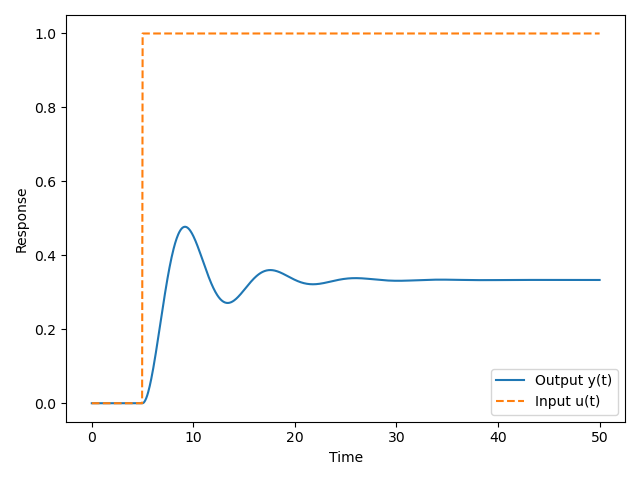
\includegraphics[scale=0.8]{../figures/mass-spring-damper-response.png}
\end{center}

Notiamo che allo stato di regime si avrà $x'' = x' = 0$ (assunta $x$ la posizione del carrello).
In questo caso la differenziale si ridurrà a:
$$
Kx = F \implies x = \frac{F}{K}
$$
che con i dati forniti dà $\sim 0.33 \, \mathrm{m}$, che come notiamo dalla figura è esattamente il punto attorno a cui il sistema si stabilizza.

\subsection{Dipendenza dalle derivate della variabile di ingresso}
Abbiamo posto finora $p = 0$, quindi nessuna derivata della variabili di ingresso.
Vediamo il caso in cui includiamo tali derivate.

\subsubsection{Caso $\mathbf{p < n}$}
Vediamo innanzitutto il caso in cui il termine di grado massimo delle variabili di stato dipende dalle derivate della variabile di ingresso, cioè $0 < p < n$.
Avevamo l'equazione differenziale:
$$
y^{(n)} (t) = \sum_{i=0}^{n-1} - \alpha_i y^{(i)}(t) + \sum_{j=0}^p \beta_j u^{(j)}(t)
$$

In questo caso la situazione si complica, e ci conviene sfruttare il \textbf{principio di sovrapposizione}.
Definiamo l'equazione ausiliaria in $z$:
$$
z^{(n)}(t) = \sum_{i = 0}^{n - 1} -\alpha_i z^{(i)}(t) + u(t)
$$
che rappresenta la risposta del sistema al solo ingresso $u(t)$ (senza derivate superiori).
Vediamo che questa è la forma che siamo stati abituati a risolvere finora.

Sarà quindi vero che la \textit{funzione forzante} (l'ingresso non scalato e non derivato) $u(t)$ porterà alla \textit{soluzione particolare} $z(t)$, cosa che indichiamo come:
$$
\mathcal{H}[u(t)] = z(t) 
$$

Considerando la linearità del sistema, siamo liberi di moltiplicare e derivare per ricavare le risposte alle funzioni derivate successive dell'ingresso scalate per i $\beta_i$ che avevamo nell'equazione originale:
\[
	\begin{cases}
		\mathcal{H}[\beta_0 u(t)] = \beta_0 z(t) \\ 
		\mathcal{H}[\beta_1 u'(t)] = \beta_1 z'(t) \\ 
		... \\
		\mathcal{H}[\beta_p u^{(p)}(t)] = \beta_p z^{(p)}(t)
	\end{cases}
\]

Per ottenere la risposta complessiva del sistema, allora, basterà applicare nuovamente la linearità e prendere la combinazione lineare delle risposte ai singoli ingressi:
$$
y(t) = \sum_{j = 0}^{p} \beta_j z^{(j)}(t)
$$
da cui il sistema finale:
\[
	\begin{cases}	
x' = \left(\begin{array}{@{}c | cccc@{}}
	0 & 1 & 0 & ... & 0 \\
	0 & 0 & 1 & ... & 0 \\
	... & ... & ... & ... & ... \\
	0 & 0 & 0 & ... & 1 \\
	\hline
	-\alpha_0 & ... & ... & ... & -\alpha_{n - 1}
\end{array}\right)
x + \begin{pmatrix}
0 \\
... \\
0 \\
1
\end{pmatrix} u \\ 
y = \begin{pmatrix}
	\beta_0 & ... & \beta_p & 0 & ... & 0
\end{pmatrix} x + \begin{pmatrix}
0
\end{pmatrix} u
	\end{cases}
\]

\subsubsection{Esempio: differenziale con derivata prima dell'ingresso}
Applichiamo il metodo appena visto per l'equazione differenziale:
$$
y'' + y = 2u + u'
$$
Notiamo il termine di derivata prima dell'ingresso $u$.
Riportandoci nella forma $y^{(n)}(t) = \hat{F}$ avremo:
$$
y'' = - y + 2u + u'
$$
con la formula al primo grado:
$$
y'' = -y + u
$$
da cui il sistema:
\[
	\begin{cases}
		\begin{pmatrix}
			x_1' \\ x_2'
		\end{pmatrix}
		=
		\begin{pmatrix}
			0 & 1 \\ 
			-1 & 0
		\end{pmatrix}
		\begin{pmatrix}
			x_1 \\ x_2
		\end{pmatrix}
		+
		\begin{pmatrix}
		0 \\ 1
		\end{pmatrix}
		u \\ 

		y = 
		\begin{pmatrix}
			2 & 1
		\end{pmatrix}
		\begin{pmatrix}
			x_1 \\ x_2
		\end{pmatrix}
		+
		\begin{pmatrix}
			0
		\end{pmatrix}
		u
	\end{cases}
\]
che sappiamo poter calcolare usando la formula di Lagrange.
In seguito vedremo un esempio di calcolo esplicito (esempio 5.0.3) per una certa configurazione di ingressi e stato iniziale.

\subsubsection{Caso $\mathbf{p = n}$}
Vediamo quindi il caso $p = n$. 
Qui avremo l'equazione differenziale:
$$
y^{(n)} (t) = \sum_{i=0}^{n-1} - \alpha_i y^{(i)}(t) + \sum_{j=0}^n \beta_j u^{(j)}(t)
$$
e la dimensione di $C$ non sarà abbastanza da contenere tutti i termini $\beta_i$.
Potremo allora definire la stessa equazione ausiliaria di prima:
$$
z^{(n)}(t) = \sum_{i = 0}^{n - 1} -\alpha_i z^{(i)}(t) + u(t)
$$
e sostituire, dopo aver preventivamente separato l'$n$-esimo termine:
$$
y(t) = \sum_{i = 1}^n \beta_{i - 1} x_i + \beta^n z^{(n)} = \sum_{i = 1}^n \beta_{i - 1} x_i + \beta_n \sum_{i = 1}^{n} -\alpha_{i - 1} z^{(i)}(t) + \beta_n u(t)
$$
da cui:
\[
	\begin{cases}	
x' = \left(\begin{array}{@{}c | cccc@{}}
	0 & 1 & 0 & ... & 0 \\
	0 & 0 & 1 & ... & 0 \\
	... & ... & ... & ... & ... \\
	0 & 0 & 0 & ... & 1 \\
	\hline
	-\alpha_0 & ... & ... & ... & -\alpha_{n - 1}
\end{array}\right)
x + \begin{pmatrix}
0 \\
... \\
0 \\
1
\end{pmatrix} u \\ 
y = \begin{pmatrix}
	\beta_0 - \beta_n \alpha_0 & ... & \beta_{n - 1} - \beta_n \alpha_{n - 1}	
\end{pmatrix} x + \begin{pmatrix}
\beta_n
\end{pmatrix} u
	\end{cases}
\]

\subsection{Rappresentazioni equivalenti}
Vediamo che la scelta di variabili di stato non è unica.
Potremmo infatti avere:
\[
	\begin{cases}
		x' = Ax + Bu \\
		y = Cx + Du
	\end{cases}
\]
e definire una matrice $T \in \mathbb{R}^{n \times n}$ invertibile detta \textbf{matrice del cambio di base} tale che:
$$
\hat{x} = Tx \implies 
\begin{cases}
	\hat{x}' = \hat{A}\hat{x} + \hat{B}u \\
	\hat{y} = \hat{C}\hat{x} + \hat{D}u
\end{cases}
$$

Ricaviamo le matrici $\hat{A}$, $\hat{B}$, $\hat{C}$ e $\hat{D}$ come:
$$
\hat{A} = T A T^{-1}, \quad \hat{B} = TB, \quad \hat{C} = CT^{-1}, \quad \hat{D} = D
$$
visto che:
\[
	\begin{cases}
		T x = T A T^{-1} T x + T B u \\ 
		y = C T^{-1} T x + D u
	\end{cases}
\]
per cancellazione di $T^{-1} T$.

Meccanicamente, questo non significa altro che possiamo prendere diversi sistemi riferimento per velocità e posizione e conservare comunque l'informazione del sistema.

\subsection{Autovalori e modi}
Avevamo dalla formula di Lagrange che per la risposta libera, cioè la soluzione di $x_l' = Ax_l$, è:
$$
	x_l(t) = e^{A(t / t_0)}x_l(t_0)
$$
posta una condizione iniziale a $t = t_0$.

Esistono 2 casi:
\begin{itemize}
	\item A \textit{diagonalizzabile};
	\item A \textit{non diagonalizzabile}.
\end{itemize}

Vediamo questi casi nel dettaglio.

\subsubsection{A diagonalizzabile}
Potremo ricavare una matrice di cambio di base $T$ tale che $A$ risulti diagonale, cioè:
$$
A = T^{-1} A_D T, \quad A_D = \begin{pmatrix}
	\lambda_1 & 0 & 0 \\
	0 & ... & 0 \\
	0 & 0 & \lambda_n
\end{pmatrix}
$$
con $A_D$ detta \textbf{matrice degli autovettori}, dove le entrate delle diagonali sono gli autovalori $A$.

In questo caso possiamo riscrivere lo stato sfruttando la serie di Taylor:
$$
\hat{x_l}(t) = e^{A_Dt} \hat{x_l}_0 = \sum_{k = 0}^\infty \frac{(A_D t)^k}{k!}\hat{x_l}_0
$$
dove la forma diagonale di $A_D$ ci permette di calcolare velocemente $A_D^k$:
$$
A_D^k = \begin{pmatrix}
	\lambda_1^k & 0 & 0 \\
	0 & ... & 0 \\
	0 & 0 & \lambda_n^k
\end{pmatrix}
$$
da cui:
$$
\hat{x_l}(t) = \mathrm{diag} \left\{ \sum_{k = 0}^\infty \frac{(\lambda_1 t)^k}{k!}, ... , \sum_{k = 0}^\infty \frac{(\lambda_n t)^k}{k!} \right\} \hat{x_l}_0
= \mathrm{diag} \left\{ e^{\lambda_1 t}, ..., e^{\lambda_n t} \right\} \hat{x_l}_0
$$
riportandoci nelle coordinate originali avremo:
$$
x_l(t) = T^{-1} \hat{x}(t) = T^{-1} \mathrm{diag} \left\{ e^{\lambda_1 t}, ..., e^{\lambda_n t} \right\} \hat{x_l}_0 = T^{-1} \mathrm{diag} \left\{ e^{\lambda_1 t}, ..., e^{\lambda_n t} \right\} T x_l(t_0)
$$

Chiamiamo gli $e^{\lambda_i}$ \textbf{modi} del sistema.
La funzioni di uscita in assenza di derivate dell'ingresso sarà quindi data da una combinazione lineare dei \textit{modi propri} del sistema:
$$
y_l(t) = C T^{-1} \mathrm{diag} \left\{ e^{\lambda_1 t}, ..., e^{\lambda_n t} \right\} T x_l(t_0)
$$

Notiamo che, come avevamo già osservato, sarà vero che $\lambda = \sigma + i \omega \in \mathbb{C}$, e quindi:
$$
e^{\lambda t} = e^{\sigma t} \cos(\omega t + \phi)
$$
dalla formula di Eulero.

\par\smallskip

Notiamo che i modi di un sistema rappresentano vari "comportamenti" naturali del sistema, che possono essere esponenziali, oscillatori o una loro combinazione sulla base del autovalore corrispondente $\lambda_i$.

Il comportamento complessivo del sistema sarà quindi dato da una qualche combinazione lineare di questi modi.

\subsubsection{A non diagonalizzabile}
Nel caso $A$ non sia diagonalizzabile si può comunque trasformare nella cosiddetta forma di \textbf{Jordan}.
Questa avrà una struttura quasi diagonale, con entrate di valore 1 immediatamente sopra la diagonale. 

In questo caso i modi assumeranno la forma:
$$
t^{\eta - 1}e^{\lambda_i} t
$$
dove $t^{\eta - 1}$ sarà un'intero compreso tra $1$ e la massima dimensione dei \textit{miniblocchi di Jordan} associati all'autovalore.

\end{document}


\documentclass[a4paper,11pt]{article}
\usepackage[a4paper, margin=8em]{geometry}

% usa i pacchetti per la scrittura in italiano
\usepackage[french,italian]{babel}
\usepackage[T1]{fontenc}
\usepackage[utf8]{inputenc}
\frenchspacing 

% usa i pacchetti per la formattazione matematica
\usepackage{amsmath, amssymb, amsthm, amsfonts}

% usa altri pacchetti
\usepackage{gensymb}
\usepackage{hyperref}
\usepackage{standalone}

% imposta il titolo
\title{Appunti Fondamenti di Automatica}
\author{Luca Seggiani}
\date{2025}

% disegni
\usepackage{pgfplots}
\pgfplotsset{width=10cm,compat=1.9}

% imposta lo stile
% usa helvetica
\usepackage[scaled]{helvet}
% usa palatino
\usepackage{palatino}
% usa un font monospazio guardabile
\usepackage{lmodern}

% tikz in sans
\tikzset{every picture/.style={/utils/exec={\sffamily}}}

\renewcommand{\rmdefault}{ppl}
\renewcommand{\sfdefault}{phv}
\renewcommand{\ttdefault}{lmtt}

% circuiti
\usepackage{circuitikz}
\usetikzlibrary{babel}

% disponi il titolo
\makeatletter
\renewcommand{\maketitle} {
	\begin{center} 
		\begin{minipage}[t]{.8\textwidth}
			\textsf{\huge\bfseries \@title} 
		\end{minipage}%
		\begin{minipage}[t]{.2\textwidth}
			\raggedleft \vspace{-1.65em}
			\textsf{\small \@author} \vfill
			\textsf{\small \@date}
		\end{minipage}
		\par
	\end{center}

	\thispagestyle{empty}
	\pagestyle{fancy}
}
\makeatother

% disponi teoremi
\usepackage{tcolorbox}
\newtcolorbox[auto counter, number within=section]{theorem}[2][]{%
	colback=blue!10, 
	colframe=blue!40!black, 
	sharp corners=northwest,
	fonttitle=\sffamily\bfseries, 
	title=Teorema~\thetcbcounter: #2, 
	#1
}

% disponi definizioni
\newtcolorbox[auto counter, number within=section]{definition}[2][]{%
	colback=red!10,
	colframe=red!40!black,
	sharp corners=northwest,
	fonttitle=\sffamily\bfseries,
	title=Definizione~\thetcbcounter: #2,
	#1
}

% disponi problemi
\newtcolorbox[auto counter, number within=section]{problem}[2][]{%
	colback=green!10,
	colframe=green!40!black,
	sharp corners=northwest,
	fonttitle=\sffamily\bfseries,
	title=Problema~\thetcbcounter: #2,
	#1
}

% disponi codice
\usepackage{listings}
\usepackage[table]{xcolor}

\lstdefinestyle{codestyle}{
		backgroundcolor=\color{black!5}, 
		commentstyle=\color{codegreen},
		keywordstyle=\bfseries\color{magenta},
		numberstyle=\sffamily\tiny\color{black!60},
		stringstyle=\color{green!50!black},
		basicstyle=\ttfamily\footnotesize,
		breakatwhitespace=false,         
		breaklines=true,                 
		captionpos=b,                    
		keepspaces=true,                 
		numbers=left,                    
		numbersep=5pt,                  
		showspaces=false,                
		showstringspaces=false,
		showtabs=false,                  
		tabsize=2
}

\lstdefinestyle{shellstyle}{
		backgroundcolor=\color{black!5}, 
		basicstyle=\ttfamily\footnotesize\color{black}, 
		commentstyle=\color{black}, 
		keywordstyle=\color{black},
		numberstyle=\color{black!5},
		stringstyle=\color{black}, 
		showspaces=false,
		showstringspaces=false, 
		showtabs=false, 
		tabsize=2, 
		numbers=none, 
		breaklines=true
}

\lstdefinelanguage{javascript}{
	keywords={typeof, new, true, false, catch, function, return, null, catch, switch, var, if, in, while, do, else, case, break},
	keywordstyle=\color{blue}\bfseries,
	ndkeywords={class, export, boolean, throw, implements, import, this},
	ndkeywordstyle=\color{darkgray}\bfseries,
	identifierstyle=\color{black},
	sensitive=false,
	comment=[l]{//},
	morecomment=[s]{/*}{*/},
	commentstyle=\color{purple}\ttfamily,
	stringstyle=\color{red}\ttfamily,
	morestring=[b]',
	morestring=[b]"
}

% disponi sezioni
\usepackage{titlesec}

\titleformat{\section}
	{\sffamily\Large\bfseries} 
	{\thesection}{1em}{} 
\titleformat{\subsection}
	{\sffamily\large\bfseries}   
	{\thesubsection}{1em}{} 
\titleformat{\subsubsection}
	{\sffamily\normalsize\bfseries} 
	{\thesubsubsection}{1em}{}

% disponi alberi
\usepackage{forest}

\forestset{
	rectstyle/.style={
		for tree={rectangle,draw,font=\large\sffamily}
	},
	roundstyle/.style={
		for tree={circle,draw,font=\large}
	}
}

% disponi algoritmi
\usepackage{algorithm}
\usepackage{algorithmic}
\makeatletter
\renewcommand{\ALG@name}{Algoritmo}
\makeatother

% disponi numeri di pagina
\usepackage{fancyhdr}
\fancyhf{} 
\fancyfoot[L]{\sffamily{\thepage}}

\makeatletter
\fancyhead[L]{\raisebox{1ex}[0pt][0pt]{\sffamily{\@title \ \@date}}} 
\fancyhead[R]{\raisebox{1ex}[0pt][0pt]{\sffamily{\@author}}}
\makeatother

\begin{document}

% sezione (data)
\section{Lezione del 05-03-25}

% stili pagina
\thispagestyle{empty}
\pagestyle{fancy}

% testo
Avevamo visto la forma standard per sistemi lineari:
\[
	\begin{cases}
		x' = Ax + Bx \\
		y = Cx + Du \\
		x(0) = x_0
	\end{cases}
\]
(con $D$ solitamente nulla), e la soluzione data da:
\[
	\begin{cases}
		x(t) = e^{At} x_0 + \int_0^t e^{A(t - \tau)} Bu(\tau) d\tau \\
		y(t) = Ce^{At} x_0 + C\int_0^t e^{A(t - \tau)} Bu(\tau) d\tau + Du \\
	\end{cases}
\]

per il calcolo di tale soluzione sfruttavamo l'\textit{esponenziale di matrice:}
$$
e^{At} = I + At + \frac{1}{2}A^2t^2+ ... + \frac{(At)^n}{n!} = \sum_{k = 0}^{+\infty} \frac{(At)^k}{k!} 
$$

Abbiamo visto che se la matrice $A$ ha autovalori distinti, allora e' diagonalizzabile:
$$
A = T^{-1} A_D T, \quad A_D = \begin{pmatrix}
	\lambda_1 & 0 & 0 \\
	0 & ... & 0 \\
	0 & 0 & \lambda_n \\
\end{pmatrix}
$$
e l'esponenziale di matrice e' semplice:
$$
e^{At} = T^{-1} e^{A_D t} T = T^{-1} \begin{pmatrix}
	e^{\lambda_1 t} & 0 & 0 \\
	0 & ... & 0 \\
	0 & 0 & e^{\lambda_n t} \\
\end{pmatrix} T
$$

In particolare, se gli autovalori sono complessi e coniugati, si avra':
$$
\lambda_i = \sigma_i + j \omega_i, \quad \overline{\lambda_i} = \sigma_i - j \omega_i 
$$
da cui:
$$
e^{\lambda_i t} = e^{\sigma_i t} e^{j\omega_i t}, \quad e^{\overline{\lambda_i} t} = e^{\sigma_i t} e^{-j\omega_i t}
$$
e si avranno quindi modi oscillatori ed esponenziali.

Avevamo inoltre definito come \textbf{modi propri} associati i:
$$
C(t) e^{\lambda t} = C(t) = \alpha_0 + \alpha_1 + \alpha_2 t^2 + ... + \alpha_{k - 1} t^{k -1}
$$

\subsubsection{Matrice reale, autovalori complessi}
Se $A$ e' reale ma i suoi autovalori sono complessi, si avra una forma del tipo:
$$
A_D = \begin{pmatrix}
	\sigma + j\omega & 0 \\
	0 & \sigma - j\omega
\end{pmatrix}
$$

Questa forma e' \textit{simile} alla matrice reale $S$:
$$
S = \begin{pmatrix}
	\sigma & \omega \\
	-\omega & \sigma
\end{pmatrix}
$$

\subsubsection{Calcolo degli autovalori}
Ripassiamo brevemente come calcolare gli autovalori.
Se $V$ e' autovettore e $\lambda$ l'autovalore associato, allora vale:
$$
Av = \lambda v \implies (A - \lambda I)v = 0 \implies \mathrm{det} (A - \lambda I) = 0
$$
detta \textbf{equazione caratteristica} $p(\lambda)$: 
$$
p(\lambda) = \mathrm{det} (A - \lambda I) = \lambda^n + \alpha_1 \lambda^{n - 1} + \alpha_2 \lambda^{n - 2} + ... + \alpha_{n - 1} \lambda + \alpha_n
$$

Avremo quindi che le soluzioni di $\lambda^*$ di $p(\lambda) = 0$ rappresentano gli autovalori di $A$.

\subsection{Forma di Jordan}
Se gli autovalori sono multipli ma $A$ non e' diagonalizzabile, abbiamo visto, occore sfruttare la \textbf{forma di Jordan} attraverso la trasformazione:
$$
J = Q A Q{-1}
$$
dove $Q$ e' la matrice degli \textbf{autovettori generalizzati} con:
$$
J = \begin{pmatrix}
	J_1 & 0 & 0 \\
	0 & ... & 0 \\
	0 & 0 & J_N
\end{pmatrix}
$$
dove ogni $J_i$ e' detto \textbf{miniblocco di Jordan}:
$$
J_i = \begin{pmatrix}
	\lambda_h & 1 & 0 & ... & 0 \\ 
	0 & \lambda_h & 1 & ... & 0 \\ 
	... & ... & ... & ... & ... \\ 
	0 & 0 & ... & \lambda_h & 1 \\
	0 & 0 & ... & 0 & \lambda_h
\end{pmatrix}
$$

Ogni blocco di Jordan ha sulla diagonale lo stesso autovalore, che compare tante volte quanto e' la sua \textit{molteplicita' algebrica}.
Inoltre, ci sono tanti blocchi $J_i$ associati allo stesso autovattore tante volte quanto e' la sua \textit{molteplicita' geometrica}.

\par\smallskip

Se riprendiamo la matrice esponenziale abbiamo:
$$
e^{At} = e^{QJQ^{-1}t} = Q \left( I + Jt + \frac{J^2 t^2}{2!} + ... + \frac{(Jt)^n}{n!} \right) Q^{-1} = Q e^{Jt} Q^{-1}
$$
dove $e^{Jt}$ e' \textit{diagonale a blocchi}:
$$
e^{Jt} = \begin{pmatrix}
e^{J_1 t} & 0 & ... & 0 \\
0 & e^{J_2 t} & ... & 0 \\
... & ... & ... & ... \\ 
0 & ... & 0 ... & e^{J_n t}
\end{pmatrix}
$$
dove ogni blocco $e^{J_i t}$ ha la forma:
$$
e^{J_i t} = e^{ \begin{pmatrix}
		\lambda & 1 & 0 \\
		0 & ... & 1 \\ 
		0 & 0 & \lambda
\end{pmatrix} t}
= e^{(\lambda I + J_{0i})t} = e^{\lambda t} e^{J_{0i} t}
$$
dove con $J_{0i}$ ci riferiamo alla \textbf{parte nilpotente} di $J_i$.
Il problema sara' quindi capire la forma di $e^{J_{0i} t}$:
$$
e^{J_{0i} t} = I + J_{0i}t + \frac{J_{0i}^2}{2!} + ... + \frac{J_{0i}^{q - i} t^{q - 1}}{(q - 1)!}
$$
dove ogni coefficiente moltiplicativo di $t^i$ ha la proprieta' di avere le entrate spostate in diagonale, verso l'alto a destra, per cui:
$$
e^{J_{0i} t} = \begin{pmatrix}
	1 & t & \frac{t^2}{2} & ... & \frac{t^{(q - 1)}}{(q - 1)!} \\
	0 & 1 & t & ... & ... \\
	0 & 0 & 1 & t & \frac{t^2}{2} \\ 
	0 & 0 & 0 & 1 & t \\
	0 & 0 & 0 & 0 & 1
\end{pmatrix}
$$
e quindi i modi del sistema sarano:
$$
t^k \frac{e^{\lambda t}}{k!}, \quad 0 \leq k \leq q - 1
$$
dove abbiamo finalmente capito il significato dell'intero $k$.

\par\smallskip
Notiamo che la proprieta' di similarita' che avevamo trovato:
$$
M = \begin{pmatrix}
	\sigma + j\omega & 0 \\
	0 & \sigma - j\omega
\end{pmatrix}
\sim
S = \begin{pmatrix}
	\sigma & \omega \\
	-\omega & \sigma
\end{pmatrix}
$$
ha un equivalente per le matrici in forma di Jordan:
$$
M=
\begin{pmatrix}
	\sigma + j \omega & 1 & 0 & 0 \\
	0 & \sigma + j \omega & 0 & 0 \\
	0 & 0 & \sigma - j \omega & 1 \\
	0 & 0 & 0 & \sigma - j \omega
\end{pmatrix}
\sim 
S=
\begin{pmatrix}
	\sigma & \omega & 1 & 0 \\
	-\omega & \sigma & 0 & 1 \\
	0 & 0 & \sigma & \omega \\
	0 & 0 & -\omega & \sigma \\
\end{pmatrix}
$$

e via dicendo.

\subsection{Stabilit' nei sistemi lineari stazionari}
Riprendiamo la definizione di \textit{stabilita'} (3.3 e 3.4).
Quello che interessa sono le \textbf{perturbazioni} dello stato.

Per un sistema lineare e stazionario l'origine e' sempre punto di equilibrio per ingresso nullo.
Se l'origine e' stabile, allora lo e' qualsiasi altro punto di equilibrio.
Si puo' allore dire che un sistema e' \textbf{stabile} solo guardando alla risposta \textit{libera} del sistema:
$$
x' = Ax + Bu, \quad u = 0, \quad x(0) = x_0
$$
$$
x(t) = e^{At}x_0
$$

In particolare, la stabilita' del sistema dipende dai \textit{modi propri} del sistema.
In particolare, se gli autovalori hanno parte reale $\mathrm{Re}(\lambda_i) < 0$ il sistema e' \textbf{asintoticamente stabile}, mentre se hanno parte reale $\mathrm{Re}(\lambda_i) \leq 0$ e gli $\mathrm{Re}(\lambda_i) = 0$ hanno molteplicita' $\mu =1$ il sistema e' solo \textbf{stabile}.
Quest'ultimo caso e' propriamente quello delle matrici non diagonalizzabili (quindi messe in forma di Jordan).

Possiamo riassumere la relazione fra stabilita', modi e autovalori come segue:
\begin{table}[H]
	\center \rowcolors{2}{white}{black!10}
	\begin{tabular} { p{3.5cm} | p{5cm} | p{5cm} }
		\bfseries Stabilita' & \bfseries Modi & \bfseries Autovalori \\
		\hline
		Stabilita' asintotica & Tendono a zero & $\mathrm{Re}(\lambda_i) < 0$ \\
	Stabilita' semplice o marginale & Non vanno a infinito, ma almeno uno non converge a zero & $\mathrm{Re}(\lambda_i) \leq 0$, $\exists \lambda_i^* : \mathrm{Re}(\lambda_i^*) = 0$, $\mu = 1$ \\
Instabilita' & Almeno uno va a infinito & $\mathrm{Re}(\lambda_i) > 0$ o $\exists \lambda_i^* : \mathrm{Re}(\lambda_i^*)$, $\mu_a(\lambda_i^*) \neq \mu_g(\lambda_i^*)$ \\
	\end{tabular}
\end{table}

\subsubsection{Stabilita' dei sistemi linearizzati}
Avevamo visto che nei sistemi non lineari conviene \textit{linearizzare} trascurando i termini oltre il primo ordine nell'intorno di uno stato di equilibrio noto.
Se il sistema linearizzato e' \textit{asintoticamente stabile}, si avra' che lo stato di equilibrio del sistema non lineare e' \textbf{stabile}.
Di contro, se il sistema linearizzato e' \textit{semplicemente stabile} non possiamo concludere nulla sul sistema non lineare (potrebbero esserci instabilita' ai termini superiori).

\end{document}


\documentclass[a4paper,11pt]{article}
\usepackage[a4paper, margin=8em]{geometry}

% usa i pacchetti per la scrittura in italiano
\usepackage[french,italian]{babel}
\usepackage[T1]{fontenc}
\usepackage[utf8]{inputenc}
\frenchspacing 

% usa i pacchetti per la formattazione matematica
\usepackage{amsmath, amssymb, amsthm, amsfonts}

% usa altri pacchetti
\usepackage{gensymb}
\usepackage{hyperref}
\usepackage{standalone}

% imposta il titolo
\title{Appunti Fondamenti di Automatica}
\author{Luca Seggiani}
\date{2025}

% disegni
\usepackage{pgfplots}
\pgfplotsset{width=10cm,compat=1.9}

% imposta lo stile
% usa helvetica
\usepackage[scaled]{helvet}
% usa palatino
\usepackage{palatino}
% usa un font monospazio guardabile
\usepackage{lmodern}

% tikz in sans
\tikzset{every picture/.style={/utils/exec={\sffamily}}}

\renewcommand{\rmdefault}{ppl}
\renewcommand{\sfdefault}{phv}
\renewcommand{\ttdefault}{lmtt}

% circuiti
\usepackage{circuitikz}
\usetikzlibrary{babel}

% disponi il titolo
\makeatletter
\renewcommand{\maketitle} {
	\begin{center} 
		\begin{minipage}[t]{.8\textwidth}
			\textsf{\huge\bfseries \@title} 
		\end{minipage}%
		\begin{minipage}[t]{.2\textwidth}
			\raggedleft \vspace{-1.65em}
			\textsf{\small \@author} \vfill
			\textsf{\small \@date}
		\end{minipage}
		\par
	\end{center}

	\thispagestyle{empty}
	\pagestyle{fancy}
}
\makeatother

% disponi teoremi
\usepackage{tcolorbox}
\newtcolorbox[auto counter, number within=section]{theorem}[2][]{%
	colback=blue!10, 
	colframe=blue!40!black, 
	sharp corners=northwest,
	fonttitle=\sffamily\bfseries, 
	title=Teorema~\thetcbcounter: #2, 
	#1
}

% disponi definizioni
\newtcolorbox[auto counter, number within=section]{definition}[2][]{%
	colback=red!10,
	colframe=red!40!black,
	sharp corners=northwest,
	fonttitle=\sffamily\bfseries,
	title=Definizione~\thetcbcounter: #2,
	#1
}

% disponi problemi
\newtcolorbox[auto counter, number within=section]{problem}[2][]{%
	colback=green!10,
	colframe=green!40!black,
	sharp corners=northwest,
	fonttitle=\sffamily\bfseries,
	title=Problema~\thetcbcounter: #2,
	#1
}

% disponi codice
\usepackage{listings}
\usepackage[table]{xcolor}

\lstdefinestyle{codestyle}{
		backgroundcolor=\color{black!5}, 
		commentstyle=\color{codegreen},
		keywordstyle=\bfseries\color{magenta},
		numberstyle=\sffamily\tiny\color{black!60},
		stringstyle=\color{green!50!black},
		basicstyle=\ttfamily\footnotesize,
		breakatwhitespace=false,         
		breaklines=true,                 
		captionpos=b,                    
		keepspaces=true,                 
		numbers=left,                    
		numbersep=5pt,                  
		showspaces=false,                
		showstringspaces=false,
		showtabs=false,                  
		tabsize=2
}

\lstdefinestyle{shellstyle}{
		backgroundcolor=\color{black!5}, 
		basicstyle=\ttfamily\footnotesize\color{black}, 
		commentstyle=\color{black}, 
		keywordstyle=\color{black},
		numberstyle=\color{black!5},
		stringstyle=\color{black}, 
		showspaces=false,
		showstringspaces=false, 
		showtabs=false, 
		tabsize=2, 
		numbers=none, 
		breaklines=true
}

\lstdefinelanguage{javascript}{
	keywords={typeof, new, true, false, catch, function, return, null, catch, switch, var, if, in, while, do, else, case, break},
	keywordstyle=\color{blue}\bfseries,
	ndkeywords={class, export, boolean, throw, implements, import, this},
	ndkeywordstyle=\color{darkgray}\bfseries,
	identifierstyle=\color{black},
	sensitive=false,
	comment=[l]{//},
	morecomment=[s]{/*}{*/},
	commentstyle=\color{purple}\ttfamily,
	stringstyle=\color{red}\ttfamily,
	morestring=[b]',
	morestring=[b]"
}

% disponi sezioni
\usepackage{titlesec}

\titleformat{\section}
	{\sffamily\Large\bfseries} 
	{\thesection}{1em}{} 
\titleformat{\subsection}
	{\sffamily\large\bfseries}   
	{\thesubsection}{1em}{} 
\titleformat{\subsubsection}
	{\sffamily\normalsize\bfseries} 
	{\thesubsubsection}{1em}{}

% disponi alberi
\usepackage{forest}

\forestset{
	rectstyle/.style={
		for tree={rectangle,draw,font=\large\sffamily}
	},
	roundstyle/.style={
		for tree={circle,draw,font=\large}
	}
}

% disponi algoritmi
\usepackage{algorithm}
\usepackage{algorithmic}
\makeatletter
\renewcommand{\ALG@name}{Algoritmo}
\makeatother

% disponi numeri di pagina
\usepackage{fancyhdr}
\fancyhf{} 
\fancyfoot[L]{\sffamily{\thepage}}

\makeatletter
\fancyhead[L]{\raisebox{1ex}[0pt][0pt]{\sffamily{\@title \ \@date}}} 
\fancyhead[R]{\raisebox{1ex}[0pt][0pt]{\sffamily{\@author}}}
\makeatother

\begin{document}

% sezione (data)
\section{Lezione del 06-03-25}

% stili pagina
\thispagestyle{empty}
\pagestyle{fancy}

% testo
\subsection{Forma di Jordan con autovalori complessi e coniugati}
Nel caso si trovi $A$ matrice reale con autovalori complessi e coniugati, è possibile usare un cambio di coordinate che trasforma la matrice diagonale complessa in una matrice reale diagonale a blocchi.

Questo è il caso che abbiamo già visto di:
$$
\begin{pmatrix}
	\sigma & \omega \\
	-\omega & \sigma
\end{pmatrix}
\sim
\begin{pmatrix}
	\sigma + j\omega & 0 \\
	0 & \sigma - j \omega
\end{pmatrix}
$$
e:
$$
\begin{pmatrix}
	\sigma & \omega & 1 & 0 \\
	-\omega & \sigma & 0 & 1 \\
	0 & 0 & \sigma & \omega \\
	0 & 0 & -\omega & \sigma \\
\end{pmatrix}
\sim
\begin{pmatrix}
	\sigma + j \omega & 1 & 0 & 0 \\
	0 & \sigma + j \omega & 0 & 0 \\
	0 & 0 & \sigma - j \omega & 1 \\
	0 & 0 & 0 & \sigma - j \omega
\end{pmatrix} 
$$

In generale, quindi, abbiamo matrici di Jordan:
$$
J_r = \begin{pmatrix}
	M & I & 0 & ... & 0 \\
	0 & M & I & ... & 0 \\
	0 & ... & M & I & 0 \\ 
	0 & ... &  0 & M & I \\
	0 & ... & ... & 0 & M
\end{pmatrix}
$$
dove gli $M$ rappresentano i singoli miniblocchi:
$$
M = \begin{pmatrix}
	\sigma & \omega \\
	-\omega & \sigma
\end{pmatrix}
$$

Il numero di blocchi è quindi pari al numero di coppie di autovalori complessi coniugati.

\subsection{Raggiungibilità}
Abbiamo visto come la proprietà di stabilita dipende solo dalla struttura del sistema, e in particolare dalla sola matrice $A$.

Vediamo come in verità esistono altre proprietà che dipendono dalla struttura del sistema e che ci sono di interesse dal punto di vista della regolazione automatica.
Una di queste proprietà è la \textbf{raggiungibilità}.

Diamo quindi la definizione:
\begin{definition}{Raggiungibilità}
	Dato il sistema dinamico di ordine $n$ con $m$ ingressi e $p$ uscite:
	\[
		\begin{cases}
			x' = Ax + Bu \\
			y = Cx + Du
		\end{cases}
	\]
		allora uno stato $\overline{x}$ si dice raggiungibile se esistono un istante di tempo finito $\overline{t} > 0$ e un ingresso $\overline{u}$ definito tra $0$ e $\overline{t}$ tali che, detto $\overline{x}_f(t)$ il movimento forzato dello stato generato da $\overline{u}$, risulti che $\overline{x}_f(\overline{t}) = \overline{x}$.
\end{definition}

La proprieta di raggiungibilità degli stati divide gli stessi in due categorie: stati raggiungibili e stati non raggiungibili.

\subsubsection{Completa raggiungibilità}
Se tutti gli stati di un sistema sono raggiungibili, allora il sistema è detto \textbf{completamente raggiungibile}.

Si può verificare se un sistema è completamente raggiungible sfruttando la matrice:

$$
\mathcal{M}_\mathcal{R} = \begin{pmatrix}
	B & AB & A^B & ... & A^{n - 1}B
\end{pmatrix}
$$
e verificando se:
$$
\mathrm{rank}(\mathcal{M}_\mathcal{R}) = n
$$

Nel caso un sistema non sia completamente raggiungibile si può isolare la parte raggiungibile, cioè definire una trasformazione $T_r$ che ci porti:
$$
x' = Ax + Bu, \quad \hat{x} = T_r x \implies \hat{x}' = \hat{A} \hat{x} + \hat{B} u
$$
con:
$$
\hat{A} = \begin{pmatrix}
\hat{A}_a & \hat{A}_{ab} \\
0 & \hat{A}_b
\end{pmatrix}, \quad
\hat{B} = \begin{pmatrix}
	\hat{B}_a \\
	0
\end{pmatrix}
$$

con $\hat{A}_a \in \mathbb{R}^{n_r \times n_r}$ e $\hat{B}_a \in \mathbb{R}^{n_r \times m}$, con $n_r = \mathrm{rank}(\mathcal{M}_\mathcal{R})$.

Posto:
$$
\hat{x} = \begin{pmatrix}
	\hat{x}_r \\ 
	\hat{x}_{nr}
\end{pmatrix}
$$
si avrà svolgendo le moltiplicazioni che:
\[
	\begin{cases}
		\hat{x}_r' = \hat{A}_a \hat{x}_r + \hat{A}_{ab} \hat{x}_{nr} + \hat{B}_a u\\
		\hat{x}_{nr}' = \hat{A}_b \hat{x}_{nr}
	\end{cases}
\]
ovvero si divide lo stato in una parte raggiungibile e in una parte non raggiungibile.

\subsubsection{Ricavare la matrice $\mathbf{T_r}$}
Per ricavare la matrice di trasformazione $T_r$ basterà scegliere $n_r$ colonne linearmente indipendenti di $\mathcal{M}_\mathcal{R}$.
Ogni stato raggiungibile sarà combinazione lineare di queste colonne.
Si aggiungono poi $n - n_r$ colonne linearmente indipendenti, prese ad arbitrio.

\end{document}

\end{document}